% change draft to final when appropriate
%\documentclass[a4paper,11pt,final]{report}
\documentclass[a4paper,11pt]{report}
\title{The ABS Language Specification\\[1cm]
\large For ABS Version 1.2.0}

\date{\today \\[1em]Document Version \input{gitRevision}}

\usepackage[includeheadfoot,left=3cm, right=3cm, top=2cm, bottom=3cm]{geometry}


\usepackage{etex}  % for more tex registers
\usepackage[svgnames]{xcolor}
\usepackage{graphics}
\usepackage[final]{graphicx}                             % TODO: change to graphics?
\graphicspath{{./figures/}}

\usepackage[utf8]{inputenc}
\usepackage[T1]{fontenc} % otherwise beramono does not work as it only provides T1 fonts
\usepackage[final]{pdfpages}                             % Include pages from another PDF document
\usepackage{ifdraft}                                     % Provides test for draft or final status
                                                         % found at: http://ftp.ktug.or.kr/tex-archive/macros/latex/contrib/oberdiek/

\usepackage{pgf,pgfarrows,xcolor}                       % PDF drawing package
\usepackage{xspace}
\usepackage{stmaryrd}                    % Exciting symbols

\usepackage[inline,nomargin]{fixme}  % Notes on things yet to do.
                             % http://www.math.utah.edu/tex-archive/macros/latex/contrib/fixme/?D=A
\usepackage{float}           % More placement control on floats
\usepackage{fancyhdr}     % Custom page headers

%% Are all of these packages needed? (Copied from old abs.tex)
\usepackage{latexsym}
\usepackage{amsfonts}
%%%\usepackage{cite}

%\usepackage{alltt}
\usepackage{booktabs}      % for fancy tables in checklist at start


\usepackage{tikz}
\usetikzlibrary{matrix,arrows}
\usetikzlibrary{shapes}
\usetikzlibrary{patterns}
\usetikzlibrary{positioning}
\usetikzlibrary{calc,decorations.pathreplacing,matrix,shadows,fit} % Compiler figure

%\usetikzlibrary{snakes}
\pgfdeclarelayer{background}
\pgfsetlayers{background,main}



\usepackage{fancyheadings}

\usepackage[all]{xy}
\usepackage{subfigure}[2002/07/30]
\usepackage{comment}
\usepackage{rotating}
%\usepackage{latexsym}
\usepackage{amsmath}
\usepackage{amssymb}
%\usepackage{txfonts} %%don't use it   %% for the slanted ||
\usepackage{mathptmx} %% this one is better
%\usepackage[standard]{ntheorem}


%\usepackage{stmaryrd}
%\usepackage{wrapfig}
\message{<Paul Taylor's Proof Trees, 2 August 1996>}
%% Build proof tree for Natural Deduction, Sequent Calculus, etc.
%% WITH SHORTENING OF PROOF RULES!
%% Paul Taylor, begun 10 Oct 1989
%% *** THIS IS ONLY A PRELIMINARY VERSION AND THINGS MAY CHANGE! ***
%%
%% 2 Aug 1996: fixed \mscount and \proofdotnumber
%%
%%      \prooftree
%%              hyp1            produces:
%%              hyp2
%%              hyp3            hyp1    hyp2    hyp3
%%      \justifies              -------------------- rulename
%%              concl                   concl
%%      \thickness=0.08em
%%      \shiftright 2em
%%      \using
%%              rulename
%%      \endprooftree
%%
%% where the hypotheses may be similar structures or just formulae.
%%
%% To get a vertical string of dots instead of the proof rule, do
%%
%%      \prooftree                      which produces:
%%              [hyp]
%%      \using                                  [hyp]
%%              name                              .
%%      \proofdotseparation=1.2ex                 .name
%%      \proofdotnumber=4                         .
%%      \leadsto                                  .
%%              concl                           concl
%%      \endprooftree
%%
%% Within a prooftree, \[ and \] may be used instead of \prooftree and
%% \endprooftree; this is not permitted at the outer level because it
%% conflicts with LaTeX. Also,
%%      \Justifies
%% produces a double line. In LaTeX you can use \begin{prooftree} and
%% \end{prootree} at the outer level (however this will not work for the inner
%% levels, but in any case why would you want to be so verbose?).
%%
%% All of of the keywords except \prooftree and \endprooftree are optional
%% and may appear in any order. They may also be combined in \newcommand's
%% eg "\def\Cut{\using\sf cut\thickness.08em\justifies}" with the abbreviation
%% "\prooftree hyp1 hyp2 \Cut \concl \endprooftree". This is recommended and
%% some standard abbreviations will be found at the end of this file.
%%
%% \thickness specifies the breadth of the rule in any units, although
%% font-relative units such as "ex" or "em" are preferable.
%% It may optionally be followed by "=".
%% \proofrulebreadth=.08em or \setlength\proofrulebreadth{.08em} may also be
%% used either in place of \thickness or globally; the default is 0.04em.
%% \proofdotseparation and \proofdotnumber control the size of the
%% string of dots
%%
%% If proof trees and formulae are mixed, some explicit spacing is needed,
%% but don't put anything to the left of the left-most (or the right of
%% the right-most) hypothesis, or put it in braces, because this will cause
%% the indentation to be lost.
%%
%% By default the conclusion is centered wrt the left-most and right-most
%% immediate hypotheses (not their proofs); \shiftright or \shiftleft moves
%% it relative to this position. (Not sure about this specification or how
%% it should affect spreading of proof tree.)
%
% global assignments to dimensions seem to have the effect of stretching
% diagrams horizontally.
%
%%==========================================================================

\def\introrule{{\cal I}}\def\elimrule{{\cal E}}%%
\def\andintro{\using{\land}\introrule\justifies}%%
\def\impelim{\using{\Rightarrow}\elimrule\justifies}%%
\def\allintro{\using{\forall}\introrule\justifies}%%
\def\allelim{\using{\forall}\elimrule\justifies}%%
\def\falseelim{\using{\bot}\elimrule\justifies}%%
\def\existsintro{\using{\exists}\introrule\justifies}%%

%% #1 is meant to be 1 or 2 for the first or second formula
\def\andelim#1{\using{\land}#1\elimrule\justifies}%%
\def\orintro#1{\using{\lor}#1\introrule\justifies}%%

%% #1 is meant to be a label corresponding to the discharged hypothesis/es
\def\impintro#1{\using{\Rightarrow}\introrule_{#1}\justifies}%%
\def\orelim#1{\using{\lor}\elimrule_{#1}\justifies}%%
\def\existselim#1{\using{\exists}\elimrule_{#1}\justifies}

%%==========================================================================

\newdimen\proofrulebreadth \proofrulebreadth=.05em
\newdimen\proofdotseparation \proofdotseparation=1.25ex
\newdimen\proofrulebaseline \proofrulebaseline=2ex
\newcount\proofdotnumber \proofdotnumber=3
\let\then\relax
\def\hfi{\hskip0pt plus.0001fil}
\mathchardef\squigto="3A3B
%
% flag where we are
\newif\ifinsideprooftree\insideprooftreefalse
\newif\ifonleftofproofrule\onleftofproofrulefalse
\newif\ifproofdots\proofdotsfalse
\newif\ifdoubleproof\doubleprooffalse
\let\wereinproofbit\relax
%
% dimensions and boxes of bits
\newdimen\shortenproofleft
\newdimen\shortenproofright
\newdimen\proofbelowshift
\newbox\proofabove
\newbox\proofbelow
\newbox\proofrulename
%
% miscellaneous commands for setting values
\def\shiftproofbelow{\let\next\relax\afterassignment\setshiftproofbelow\dimen0 }
\def\shiftproofbelowneg{\def\next{\multiply\dimen0 by-1 }%
\afterassignment\setshiftproofbelow\dimen0 }
\def\setshiftproofbelow{\next\proofbelowshift=\dimen0 }
\def\setproofrulebreadth{\proofrulebreadth}

%=============================================================================
\def\prooftree{% NESTED ZERO (\ifonleftofproofrule)
%
% first find out whether we're at the left-hand end of a proof rule
\ifnum  \lastpenalty=1
\then   \unpenalty
\else   \onleftofproofrulefalse
\fi
%
% some space on left (except if we're on left, and no infinity for outermost)
\ifonleftofproofrule
\else   \ifinsideprooftree
        \then   \hskip.5em plus1fil
        \fi
\fi
%
% begin our proof tree environment
\bgroup% NESTED ONE (\proofbelow, \proofrulename, \proofabove,
%               \shortenproofleft, \shortenproofright, \proofrulebreadth)
\setbox\proofbelow=\hbox{}\setbox\proofrulename=\hbox{}%
\let\justifies\proofover\let\leadsto\proofoverdots\let\Justifies\proofoverdbl
\let\using\proofusing\let\[\prooftree
\ifinsideprooftree\let\]\endprooftree\fi
\proofdotsfalse\doubleprooffalse
\let\thickness\setproofrulebreadth
\let\shiftright\shiftproofbelow \let\shift\shiftproofbelow
\let\shiftleft\shiftproofbelowneg
\let\ifwasinsideprooftree\ifinsideprooftree
\insideprooftreetrue
%
% now begin to set the top of the rule (definitions local to it)
\setbox\proofabove=\hbox\bgroup$\displaystyle % NESTED TWO
\let\wereinproofbit\prooftree
%
% these local variables will be copied out:
\shortenproofleft=0pt \shortenproofright=0pt \proofbelowshift=0pt
%
% flags to enable inner proof tree to detect if on left:
\onleftofproofruletrue\penalty1
}

%=============================================================================
% end whatever box and copy crucial values out of it
\def\eproofbit{% NESTED TWO
%
% various hacks applicable to hypothesis list 
\ifx    \wereinproofbit\prooftree
\then   \ifcase \lastpenalty
        \then   \shortenproofright=0pt  % 0: some other object, no indentation
        \or     \unpenalty\hfil         % 1: empty hypotheses, just glue
        \or     \unpenalty\unskip       % 2: just had a tree, remove glue
        \else   \shortenproofright=0pt  % eh?
        \fi
\fi
%
% pass out crucial values from scope
\global\dimen0=\shortenproofleft
\global\dimen1=\shortenproofright
\global\dimen2=\proofrulebreadth
\global\dimen3=\proofbelowshift
\global\dimen4=\proofdotseparation
\global\count255=\proofdotnumber
%
% end the box
$\egroup  % NESTED ONE
%
% restore the values
\shortenproofleft=\dimen0
\shortenproofright=\dimen1
\proofrulebreadth=\dimen2
\proofbelowshift=\dimen3
\proofdotseparation=\dimen4
\proofdotnumber=\count255
}

%=============================================================================
\def\proofover{% NESTED TWO
\eproofbit % NESTED ONE
\setbox\proofbelow=\hbox\bgroup % NESTED TWO
\let\wereinproofbit\proofover
$\displaystyle
}%
%
%=============================================================================
\def\proofoverdbl{% NESTED TWO
\eproofbit % NESTED ONE
\doubleprooftrue
\setbox\proofbelow=\hbox\bgroup % NESTED TWO
\let\wereinproofbit\proofoverdbl
$\displaystyle
}%
%
%=============================================================================
\def\proofoverdots{% NESTED TWO
\eproofbit % NESTED ONE
\proofdotstrue
\setbox\proofbelow=\hbox\bgroup % NESTED TWO
\let\wereinproofbit\proofoverdots
$\displaystyle
}%
%
%=============================================================================
\def\proofusing{% NESTED TWO
\eproofbit % NESTED ONE
\setbox\proofrulename=\hbox\bgroup % NESTED TWO
\let\wereinproofbit\proofusing
\kern0.3em$
}

%=============================================================================
\def\endprooftree{% NESTED TWO
\eproofbit % NESTED ONE
% \dimen0 =     length of proof rule
% \dimen1 =     indentation of conclusion wrt rule
% \dimen2 =     new \shortenproofleft, ie indentation of conclusion
% \dimen3 =     new \shortenproofright, ie
%                space on right of conclusion to end of tree
% \dimen4 =     space on right of conclusion below rule
  \dimen5 =0pt% spread of hypotheses
% \dimen6, \dimen7 = height & depth of rule
%
% length of rule needed by proof above
\dimen0=\wd\proofabove \advance\dimen0-\shortenproofleft
\advance\dimen0-\shortenproofright
%
% amount of spare space below
\dimen1=.5\dimen0 \advance\dimen1-.5\wd\proofbelow
\dimen4=\dimen1
\advance\dimen1\proofbelowshift \advance\dimen4-\proofbelowshift
%
% conclusion sticks out to left of immediate hypotheses
\ifdim  \dimen1<0pt
\then   \advance\shortenproofleft\dimen1
        \advance\dimen0-\dimen1
        \dimen1=0pt
%       now it sticks out to left of tree!
        \ifdim  \shortenproofleft<0pt
        \then   \setbox\proofabove=\hbox{%
                        \kern-\shortenproofleft\unhbox\proofabove}%
                \shortenproofleft=0pt
        \fi
\fi
%
% and to the right
\ifdim  \dimen4<0pt
\then   \advance\shortenproofright\dimen4
        \advance\dimen0-\dimen4
        \dimen4=0pt
\fi
%
% make sure enough space for label
\ifdim  \shortenproofright<\wd\proofrulename
\then   \shortenproofright=\wd\proofrulename
\fi
%
% calculate new indentations
\dimen2=\shortenproofleft \advance\dimen2 by\dimen1
\dimen3=\shortenproofright\advance\dimen3 by\dimen4
%
% make the rule or dots, with name attached
\ifproofdots
\then
        \dimen6=\shortenproofleft \advance\dimen6 .5\dimen0
        \setbox1=\vbox to\proofdotseparation{\vss\hbox{$\cdot$}\vss}%
        \setbox0=\hbox{%
                \advance\dimen6-.5\wd1
                \kern\dimen6
                $\vcenter to\proofdotnumber\proofdotseparation
                        {\leaders\box1\vfill}$%
                \unhbox\proofrulename}%
\else   \dimen6=\fontdimen22\the\textfont2 % height of maths axis
        \dimen7=\dimen6
        \advance\dimen6by.5\proofrulebreadth
        \advance\dimen7by-.5\proofrulebreadth
        \setbox0=\hbox{%
                \kern\shortenproofleft
                \ifdoubleproof
                \then   \hbox to\dimen0{%
                        $\mathsurround0pt\mathord=\mkern-6mu%
                        \cleaders\hbox{$\mkern-2mu=\mkern-2mu$}\hfill
                        \mkern-6mu\mathord=$}%
                \else   \vrule height\dimen6 depth-\dimen7 width\dimen0
                \fi
                \unhbox\proofrulename}%
        \ht0=\dimen6 \dp0=-\dimen7
\fi
%
% set up to centre outermost tree only
\let\doll\relax
\ifwasinsideprooftree
\then   \let\VBOX\vbox
\else   \ifmmode\else$\let\doll=$\fi
        \let\VBOX\vcenter
\fi
% this \vbox or \vcenter is the actual output:
\VBOX   {\baselineskip\proofrulebaseline \lineskip.2ex
        \expandafter\lineskiplimit\ifproofdots0ex\else-0.6ex\fi
        \hbox   spread\dimen5   {\hfi\unhbox\proofabove\hfi}%
        \hbox{\box0}%
        \hbox   {\kern\dimen2 \box\proofbelow}}\doll%
%
% pass new indentations out of scope
\global\dimen2=\dimen2
\global\dimen3=\dimen3
\egroup % NESTED ZERO
\ifonleftofproofrule
\then   \shortenproofleft=\dimen2
\fi
\shortenproofright=\dimen3
%
% some space on right and flag we've just made a tree
\onleftofproofrulefalse
\ifinsideprooftree
\then   \hskip.5em plus 1fil \penalty2
\fi
}

%==========================================================================
% IDEAS
% 1.    Specification of \shiftright and how to spread trees.
% 2.    Spacing command \m which causes 1em+1fil spacing, over-riding
%       exisiting space on sides of trees and not affecting the
%       detection of being on the left or right.
% 3.    Hack using \@currenvir to detect LaTeX environment; have to
%       use \aftergroup to pass \shortenproofleft/right out.
% 4.    (Pie in the sky) detect how much trees can be "tucked in"
% 5.    Discharged hypotheses (diagonal lines).

\usepackage{varioref}
%\usepackage{ifthen}
\renewcommand{\vref}[1]   {\ref{#1}}


\usepackage[final]{listings}
\lstset{mathescape}
\lstset{basicstyle=\scriptsize}
\lstset{numberstyle=\tiny}%
\lstset{language=}
%\lstset{numbers=left,numberstyle=\tiny,stepnumber=5}
%\lstset{frame=trBL} %% The evil frame

\lstset{emphstyle=\color{red},emphstyle={[2]\color{blue}\underbar}}%% global

%>> \usepackage{pstricks,pst-node,pst-text,pst-3d} for scalebox


%\usepackage{lstoc}
%\lstset{language=Oc}
\usepackage{psfrag}



%\usepackage{changebar}
\usepackage{longtable}

\usepackage[scaled=.83]{beramono} % nicer tt font
%\usepackage{helvet}               % nicer sf font

%\usepackage{beramono}
%\usepackage{courier}
%\usepackage{listings}

%%%%%%%%%%%%%%%%%%%%%%%%%%%%%%%%%%%%%%%%%%%%%%%%%%%%%%%%%%%%%%%%%%%%%%%%%%%%%%%%%%%%%%%%%%%%%%%%

%%% Hyperref customization for PDF presentation
\usepackage[unicode]{hyperref}      % Insert hyperlinks and talk unicode
                                    % to pdflatex.  Keep this package last.

\hypersetup {
  bookmarksopen=true,     % When bookmarks shown, unfold them
  bookmarksopenlevel=0,   % Show chapters (0) only
  bookmarksnumbered=true, % Include section numbers
  pdftitle =                 % Text form of title
                 { The ABS Language Specification },
  pdfauthor=              % Text form of author
                { HATS Project },
}


%%% Local Variables:
%%% mode: LaTeX
%%% TeX-master: "absrefmanual"
%%% End:

%%%%%%%%%%%%%%%%%%%%%%%%%%%%%%%%%%%%%%%%%%%%%%%%%%%%%%%%%%%%
% some commonly used commands

\definecolor{darkblue}{rgb}{0,0,0.6}
\definecolor{darkgreen}{rgb}{0,0.6,0}
\definecolor{darkred}{rgb}{0.7,0,0}

\newcommand{\mynote}[1]{
  \ensuremath{\left\langle\right.\!\!\left\langle\right.\!}\bf #1%
  \ensuremath{\!\left.\right\rangle\!\!\left.\right\rangle}}
\newcommand{\DC}[1]{\textcolor{blue}{\mynote{DC: #1}}}
\newcommand{\RM}[1]{\textcolor{darkgreen}{\mynote{RM: #1}}}
\newcommand{\JP}[1]{\textcolor{darkred}{\mynote{JP: #1}}}
\newcommand{\JS}[1]{\textcolor{violet}{\mynote{JS: #1}}}

\newcommand{\muTVL}{\ensuremath{\mu\textrm{TVL}}\xspace}
\newcommand{\fid}{\ensuremath{\mathsf{FID}}\xspace}
\newcommand{\aid}{\ensuremath{\mathsf{AID}}\xspace}
\newcommand{\name}{\ensuremath{\mathsf{Name}}\xspace}

%%%%%%%%%%%%%%%%%%%%%%%%%%%%%%%%%%%%%%%%%%%%%%%%%%%%%%%%%%%%
%% Concrete syntax used in D1.2

\newcommand{\NT}[1]{\textit{#1}}
%\newcommand{\TR}[1]{\texttt{\underline{\raisebox{-2.2pt}{\rule{0pt}{0pt}}#1}}}
\newcommand{\TR}[1]{\ensuremath{\mathtt{#1}}}
\newcommand{\TRS}[1]{\texttt{#1}}
\newcommand{\VAR}[1]{\textsc{#1}}
%\newcommand{\MANY}[1]{\ensuremath{\bnfmany{#1}}}
%\newcommand{\MANYG}[1]{\ensuremath{\bnfmany{(#1)}}}
\newcommand{\MANY}[1]{#1\ensuremath{^*}}
\newcommand{\MANYG}[1]{\ensuremath{(}#1\ensuremath{)^*}}
\newcommand{\PLUS}[1]{\bnfplus{#1}}
\newcommand{\PLUSG}[1]{\bnfplus{(#1)}}
\newcommand{\OPT}[1]{\ensuremath{[}#1\ensuremath{]}}
\newcommand{\OPTG}[1]{\ensuremath{[}#1\ensuremath{]}}
%\raisebox{-2pt}{\rule{0pt}{0pt}

%\newcommand{\defNT}[1]{\NT{#1} &::=&}
\newcommand{\defn}{&::=&}
\newcommand{\defc}{\\&\multicolumn{1}{r}{\ensuremath{|}}&}
\newcommand{\concrDefn}[1]{\defn #1}
\newcommand{\concrCont}[1]{\defc #1}
\newcommand{\concrNewline}[1]{\\&& #1}


\newenvironment{bnfgrammar}
{\begin{tabular}{lrl@{\hspace{3mm}}l}}
{\end{tabular}}

\newenvironment{abssyntax}
{~\\[1ex]\noindent\textbf{Syntax:}\\[1ex]
\begin{bnfgrammar}}
{\end{bnfgrammar}\\[1ex]}

\newenvironment{abstractgrammar}
{\[ \begin{array}[t]{@{}lrl@{\hspace{3mm}}l@{}}}
{\end{array}\]}

%%%%%%%%%%%%%%%%%%%%%%%%%%%%%%%%%%%%%%%%%%%%%%%%%%%%%%%%%%%%
%% Making grammars consistent

\newcommand{\bnfoptional}[1]     {{ [} #1 { ]}\, }
\newcommand{\bnfplus}[1]{#1\ensuremath{^+}}%one or more occurrences, separated by comma
\newcommand{\bnfdef}               {::=}
\newcommand{\bnfbar}               {\mathrel{|}}

\newcommand{\seqof}[1]{\MANY{#1}}
\newcommand{\bnfmany}[1]{\MANY{#1}}
\newcommand{\many}[1]{\MANY{#1}}
\newcommand{\manymath}[1]{\ensuremath{\overline{#1}}}
\newcommand{\kw}[1]{\ensuremath{\mathtt{#1}}}  % same as \TR

\newcommand{\seqofg}[1]{\MANYG{#1}}
\newcommand{\bnfmanyg}[1]{\MANYG{#1}}
\newcommand{\manyg}[1]{\MANYG{#1}}

\newcommand{\grshape}{\slshape}
%\newcommand{\grface}{\texttt}

\newcommand{\gmany}[1]     {\{#1\}}                      %%% 
%\newcommand{\gopt}[1] {\textup{[}{#1}\textup{]}}
\newcommand{\gopt}[1] {[{#1}]}
\newcommand{\gbar}{\ensuremath{|\ }}
\newcommand{\posix}[1]     {\textup{[:\,}{#1}\textup{\,:]}}                      %%% 

%\newcommand{\grface}{\textsl}
%\newcommand{\grface}{\texttt}

\newcommand{\sourcefont}{\ttfamily}
\newcommand{\commentfont}{\slshape\rmfamily\color{black!70}}

%%%%%%%%%%%%%%%%%%%%%%%%%%%%%%%%%%%%%%%%%%%%%%%%%%%%%%%%%%%%

\colorlet{keywordcolor}{blue!50!black}

\lstdefinelanguage{ABS}{
 language=Java,
 deletekeywords={void,long,int,byte,boolean,true,false}, 
 morekeywords={type, data, def, cog, export, import, get, let, then, in, await, assert,suspend,module,from,now,duration,deadline,
delta,uses,adds,modifies,removes,original,core,productline,corefeatures,optionalfeatures,after,when,product,hasAttribute,hasMethod},
}

%\def\codesize{\fontsize{9}{10}}

\lstnewenvironment{abs}{%
  \lstset{language=ABS,columns=fullflexible,mathescape=true,%
           keywordstyle=\bf\sffamily,commentstyle=\sl\sffamily,%
           basicstyle=\footnotesize\normalfont\sffamily,inputencoding=latin1, % i would prefer utf8
           extendedchars,xleftmargin=2em,showstringspaces=false}%
  \csname lst@SetFirstLabel\endcsname}
  {\csname lst@SaveFirstLabel\endcsname}


%%%% mTVL
\lstdefinelanguage{MTVL}{keywords=
{root,group,extension,oneof,allof,opt},
  sensitive=true,
  morecomment=[l]{//},
  morestring=[b]"}

%\def\codesize{\fontsize{9}{10}}
\lstnewenvironment{mtvl}{%
 \lstset{language=MTVL,columns=fullflexible,mathescape=true,%
           keywordstyle=\bf\sffamily,commentstyle=\sl\sffamily,%
           basicstyle=\footnotesize\normalfont\sffamily,inputencoding=latin1, % i would prefer utf8
           extendedchars,xleftmargin=2em}%
   \csname lst@SetFirstLabel\endcsname}
  {\csname lst@SaveFirstLabel\endcsname}

%%%% Spec lang

\lstdefinelanguage{SPEC}{keywords={interface,spec,in,out,calls,returns},
  sensitive=true,
  comment=[l]{//},
  morecomment=[s]{/*}{*/},
  morestring=[b]"}
\lstnewenvironment{spec}{%
\lstset{language=SPEC,columns=fullflexible,mathescape=true,%
        keywordstyle=\bf\sffamily,commentstyle=\sl\sffamily,%
        basicstyle=\footnotesize\normalfont\sffamily,inputencoding=latin1, % i would prefer utf8
        extendedchars,xleftmargin=2em}%
  \csname lst@SetFirstLabel\endcsname}
  {\csname lst@SaveFirstLabel\endcsname}

\lstdefinestyle{absgrammar}{
  basicstyle=\ttfamily,
%  moredelim=[is][\bfseries]{'}{'},
%  morecomment=[s][\bfseries]{'}{'},
%  stringstyle=\bfseries,
  morestring=[b]',
  columns = fullflexible,%spaceflexible,%fullflexible,
  columns = fixed,
  fontadjust = true,
  keepspaces = true, % do not summarize spaces
  mathescape={false},
  xleftmargin=1.5em,
 showstringspaces = false,
}

\lstdefinestyle{absnobg} {
 language=ABS,
 basicstyle=\sourcefont\upshape,
 commentstyle=\commentfont,
 keywordstyle=\bfseries\color{keywordcolor}\upshape,
% deletekeywords={static,public,private}
 classoffset=1,
 % standard types:
 morekeywords={Unit,Int, Rat, Bool, List, Set, Pair, Fut, Maybe, String, Triple, Either, Map},
 keywordstyle=\color{violet},
 classoffset=0,
 mathescape={true},
 escapechar={\#},
 columns = fullflexible,%spaceflexible,%fullflexible,
 fontadjust = true,
 keepspaces = true, % do not summarize spaces
 showstringspaces = false,
% inputencoding=utf8,
% numbers=left,
 xleftmargin=1.5em,
framexleftmargin=1em,
framextopmargin=0.5ex,
% breaklines=true,
% lineskip=0pt, 
% abovecaptionskip=-1ex,
% belowcaptionskip=-1ex,
% breakautoindent = true,
% breakindent = 2em,
% breaklines = true,
 emptylines=10
}

\lstdefinestyle{abs} {
style=absnobg,
framerule=1pt,
backgroundcolor=\color{blue!5},
rulecolor=\color{gray!50},
frame=tblr
}

% make abs the default style
%\lstset{
%style=abs
%}

\lstdefinestyle{absexample}{
style=abs,
%backgroundcolor=\color{green!80!black!10},
}

\newcommand{\absinline}[1]{\lstinline[style=abs]{#1}}
\newcommand{\absinlinesmall}[1]{\lstinline[style=abs,basicstyle=\sourcefont\footnotesize\upshape,
 commentstyle=\commentfont\footnotesize,
 keywordstyle=\bfseries\color{keywordcolor}\footnotesize\upshape]{#1}}

\lstnewenvironment{abscode}{
\lstset{style=abs}}
{}

\lstnewenvironment{abscodesmall}{
\lstset{style=abs, basicstyle=\sourcefont\footnotesize\upshape,
 commentstyle=\commentfont\footnotesize,
 keywordstyle=\bfseries\color{keywordcolor}\footnotesize\upshape
}}
{}

\lstnewenvironment{abscodesmallnobg}{
\lstset{style=absnobg, basicstyle=\sourcefont\footnotesize\upshape,
 commentstyle=\commentfont\footnotesize,
 keywordstyle=\bfseries\color{keywordcolor}\footnotesize\upshape
}}
{}

\lstnewenvironment{absgrammar}{%
~\\[1ex]\noindent\textbf{Syntax:}
\lstset{style=absgrammar}}
{}



%%%%%%%%%%%%%%%%%%%%%%%%%%%%%%%%%%%%%%%%%%%%%%%%%%%%%%%%%%%%

\newcommand{\grsh}[1]{{\grshape #1}}

\newenvironment{grprode}[2]
{{\grshape #1}\,:
\\\indent\indent{\grshape #2}}
{\vspace{.75\baselineskip}}

\newcommand{\gprod}[2]{\begin{grprode}{#1}{#2}\end{grprode}}   
\newcommand{\gnewline}{\\\mbox{}\hspace{4em}}   


\newcommand{\gexnewline}{\\\mbox{}\indent}   

%\newcommand{\gnlbar}{\gnewline\mbox{}\hspace{-1em}\gbar}
%or
\newcommand{\gnlbar}{\gnewline\gbar}

\lstnewenvironment{absexample}
{\subsubsection*{Example:}
\lstset{style=absexample}}
{}

\newcommand{\kwdecl}{\upshape\ttfamily}
\newcommand{\mcode}[1]{{\texttt{#1}}} %mycode

\newcommand{\kwlbrace} {\kw{\{\,}}
\newcommand{\kwrbrace} {\kw{\}}}
\newcommand{\kwlparen} {\kw{(\,}}
\newcommand{\kwrparen} {\kw{)}}
\newcommand{\kwdot} {\kw{.}}

\newcommand{\kwassign} {$\,\kw{=}\,$}
\newcommand{\kwsemi} {$\,\kw{;}\,$}
\newcommand{\kwbar} {$\,\kw{|}\,$}
\newcommand{\kwcomma} {$\,\kw{,}\,$}
\newcommand{\kwlt} {$\,\kw{<}$}
\newcommand{\kwgt} {$\kw{>}\,$}
\newcommand{\kwclass} {\kw{class}}
\newcommand{\kwinterface} {\kw{interface}}
\newcommand{\kwextends} {\kw{extends}}
\newcommand{\kwdata} {\kw{data}}
\newcommand{\kwdef} {\kw{def}}
\newcommand{\kwimplements} {\kw{implements}}
\newcommand{\kwwhile} {\kw{while}}
\newcommand{\kwassert} {\kw{assert}}
\newcommand{\kwreturn} {\kw{return}}
\newcommand{\kwfut} {\kw{Fut}}
\newcommand{\kwskip} {\kw{skip}}
\newcommand{\kwget} {\kw{get}}
\newcommand{\kwnull} {\kw{null}}
\newcommand{\kwawait} {\kw{await}}
\newcommand{\kwif} {\kw{if}}
\newcommand{\kwthen} {\kw{then}}
\newcommand{\kwelse} {\kw{else}}
\newcommand{\kwsuspend} {\kw{suspend}}
\newcommand{\kwnew} {\kw{new}}
\newcommand{\kwthis} {\kw{this}}
\newcommand{\kwcase} {\kw{case}}
\newcommand{\kwlet} {\kw{let}}
\newcommand{\kwin} {\kw{in}}
\newcommand{\kwcog} {\kw{cog}}
\newcommand{\kwtype} {\kw{type}}
\newcommand{\kwguardand} {\kw{\&}}
\newcommand{\kwbang} {\kw{!}}


%%%%%%%%%%%%%%%%%%%%%%%%%%%%%%%%%%%%%%%%%%%%%%%%%%%%%%%%%%%%
%% tikz styles

\tikzstyle{box} = [draw=black,thick,bottom color=black!20,top color=white]
\tikzstyle{bx2} = [draw=black,thick,bottom color=blue!40,top color=white]
\tikzstyle{art} = [draw=black,rounded corners=7pt, thick,
  fill=blue!20, text=black, inner sep=2mm,font=\sffamily]
\tikzstyle{art2}= [art, bottom color=blue!10!gray!40, top color=white]


\pgfdeclarelayer{background}
\pgfdeclarelayer{cogs}
\pgfdeclarelayer{main}
\pgfsetlayers{background,cogs,main}


\newcommand{\diagramfont}{\sffamily}
\tikzstyle{lightshadow}=[drop shadow={shadow scale=1, fill=black!20,
%opacity=.5,
shadow xshift=1.2pt, shadow yshift=-1.2pt}]

\tikzstyle{ultralightshadow}=[
drop shadow={shadow scale=1, fill=black!10,
shadow xshift=2.5pt, shadow yshift=-2.5pt}]

\tikzstyle{diagramnodeWithoutShadow}=[draw=black!50,fill=white,font=\diagramfont,
line width=0.8pt, text depth=0ex]

\tikzstyle{diagramnode}=[diagramnodeWithoutShadow,
lightshadow]


\tikzstyle{object}=[diagramnode,rectangle,rounded corners=2pt,
inner sep=2mm,fill=black!2,fill=Lavender!80,%fill=blue!20!white,
%shadow xshift=0.2ex, shadow yshift=-0.2ex}
%path fading=south, shading angle=45}
]
\tikzstyle{mainobject}=[object,font=\diagramfont\bfseries]
\tikzstyle{cogform}=[rectangle,line width=1.5pt,draw=black!20,
text depth=0ex,inner sep=6pt,rounded corners]
\tikzstyle{cog}=[cogform, ultralightshadow, fill=black!2,
%draw=blue!50,fill=blue!10,
] % inner sep = 0.45cm

\tikzstyle{legendtext}=[right,text depth=0,font=\diagramfont\footnotesize]
\tikzstyle{legendsymbol}=[left,text depth=0,font=\diagramfont\footnotesize]

\tikzstyle{myarrow}=[single arrow,draw=gray!25,fill=gray!10,very thick]


%%% Local Variables: 
%%% mode: latex
%%% TeX-master: "main"
%%% End: 

%%%% command line snippets
\lstdefinelanguage{cmdline}{
    keywords={},
    sensitive=true,
%     comment=[l]{//},
%     morecomment=[s]{/*}{*/},
    morestring=[b]"
}

\lstdefinestyle{cmdstyle}{
    language=cmdline,
    columns=fullflexible,
    mathescape=false,
    showstringspaces=false,
    keywordstyle=\bf\sffamily,
    commentstyle=\sl\sffamily,
    basicstyle=\normalsize\ttfamily,
    inputencoding=latin1,
    extendedchars,
    xleftmargin=4pt,
    xrightmargin=4pt,
    breaklines=true,
    breakatwhitespace=true
%    keepspaces=false,
%    resetmargins=true
}

\lstnewenvironment{cmdline}[1][]{
    \lstset{style=cmdstyle,#1}
    \csname lst@SetFirstLabel\endcsname}
{\csname lst@SaveFirstLabel\endcsname}

\newcommand{\cmd}[1]{\lstset{style=cmdstyle}\lstinline!#1!}



\def\codesize{\fontsize{8}{8}}
\newcommand{\CT}{\env{\mathcal{C}}}


\begin{document}

\maketitle

\tableofcontents

\chapter{Introduction}
This chapter describes the core ABS language as it is implemented in
the ABS tools.  The ABS language is a class-based object-oriented
language that features algebraic data types and side effect-free
functions.  Syntactically, the ABS language tries to be as close as
possible to the Java language~\cite{gosling96} so that programmers
that are used to Java can easily use the ABS language without much
learning effort.

\section{Notation}
In this chapter we often present the concrete syntax of the ABS language.\index{syntax}
To do so we use BNF\footnote{Backus-Naur Form} with the following denotations.
\begin{itemize}
\item $\OPT{x}$ denotes zero or one occurrence of $x$. \\
The same notation is used to represent an optional element in the formal system.
In effect $\OPT{x}$ corresponds to either nothing or an element of $x$.
\item $\MANY{x}$ denotes zero or more occurrences of $x$. \\
Note that in formal semantics the notation $\manymath{x}$ is used to
 represent an explicit sequence of elements $x_1,\ldots,x_n$; similarly $\manymath{x}:\manymath{T}$ represents
$x_1:T_1,\ldots,x_n:T_n$, following Pierce~\cite{Pierce:TypeSystems}.
\item $\PLUS{x}$ denotes one or more occurrences of $x$.
\item $x \bnfbar y$ means one of either $x$ or $y$.
\item \posix{$x$} denotes the POSIX character class $x$. %\todo{reference to POSIX}
%\item \verb_'x'_ denotes that \verb_x_ is a terminal symbol
%\item \bnfplus{x} denotes one or more occurrences of x. 
\item text in \TR{monospace} denotes terminal symbols.
\item text in \NT{italics} denotes non-terminals in the grammar.
%\item text in \textsf{sans serif} font denotes identifiers in an abstract grammar.
\end{itemize}

\chapter{Lexical Structure}
\label{ch:lexical structure}
This section describes the lexical structure of the ABS language.
ABS programs are written in Unicode.\footnote{\url{http://www.unicode.org}}

\section{Line Terminators and White Spaces}
Line terminators and white spaces are defined as in Java.
%\begin{absgrammar}
%LineTerminator ::= \n | \r | \r\n
%WhiteSpace     ::= LineTerminator | ' ' | \t | \f
%\end{absgrammar}
%
\begin{abssyntax}
\NT{LineTerminator}
\concrDefn{} \verb_\_\TR{n}  ~|~ \verb_\_\TR{r} ~|~ \TR{rn} 
\\
\NT{WhiteSpace} \concrDefn{}
  \NT{LineTerminator} ~|~ \verb*_ _ ~|~ \verb_\_\TR{t} ~|~ \verb_\_\TR{f}
\end{abssyntax}

\section{Comments}
Comments are code fragments that are completely ignored and have no semantics in the ABS language.
ABS supports two styles of comments:
\emph{end-of-line comments} and \emph{traditional comments}.

\subsection{End-Of-Line Comments}
An end-of-line comment is a code fragment that starts with two slashes, e.g., \verb_// text_. All text that follows \verb_//_ until the end of the line is treated as a comment.

\begin{absexample}
// this is a comment
module A; // this is also a comment
\end{absexample}

\subsection{Traditional Comments}
A traditional comment is a code fragment that is enclosed in \absinline{/* */}, e.g., \absinline{/* this is a comment */}.
Nested traditional comments are not possible.

\begin{absexample}
/* this
is a multiline
comment */  
\end{absexample}


\section{Identifiers}
ABS distinguishes \emph{identifier} and \emph{type identifier}.
They differ in the first character, which must be a lower-case character
for identifiers and an upper-case character for type identifiers.
%
%\begin{absgrammar}
%Identifier     ::= [:lowercase:] {[:letter:] | [:digit:] | '_'}
%TypeId         ::= [:uppercase:] {[:letter:] | [:digit:] | '_'}
%\end{absgrammar}
%
\begin{abssyntax}
\NT{Identifier}  \defn
  \text{[:lower:]} \MANYG{\text{[:alpha:] ~|~ [:digit:] ~|~ \TR{\_}}}
\\
\NT{TypeId}      \defn
  \text{[:upper:]} \MANYG{\text{[:alpha:] ~|~ [:digit:] ~|~ \TR{\_}}}
\end{abssyntax}

\section{Keywords}
The following words are keywords in the ABS language and are \emph{not}
regarded as identifiers.

\noindent
\begin{center}
\begin{tabular}{llllll}
\TR{adds} & \TR{after} & \TR{assert} & \TR{await} & \TR{builtin} & \TR{case} \\
\TR{cog} & \TR{core} & \TR{class} & \TR{data} & \TR{def} & \TR{delta} \\
\TR{else} & \TR{export} & \TR{features} & \TR{from} & \TR{get} & \TR{hasField} \\
\TR{hasInterface} & \TR{hasMethod} & \TR{if} & \TR{implements} & \TR{import} & \TR{in} \\
\TR{interface} & \TR{let} & \TR{modifies} & \TR{module} & \TR{new} & \TR{null} \\
\TR{product} & \TR{productline} & \TR{removes} & \TR{return} & \TR{skip} & \TR{suspend} \\
\TR{this} & \TR{type} & \TR{when} & \TR{while} & &\\ 
\end{tabular}
\end{center}

\section{Literals}
A \emph{literal} is a textual representation of a value.
ABS supports three kinds of literals, \emph{integer literals}, \emph{string literals}, and the \emph{null literal}.

\begin{abssyntax}
\NT{Literal}       \defn \NT{IntLiteral}
                ~|~ \NT{StringLiteral}
                ~|~ \NT{NullLiteral}
                \\
\NT{IntLiteral}    \defn 0 ~|~ [1-9]\MANY{[0-9]}\\
\NT{StringLiteral} \defn \TR{"} \MANY{\NT{StringCharacter}} \TR{"}\\
\NT{NullLiteral}   \defn \TR{null}
\end{abssyntax}

\noindent
Where a \NT{StringCharacter} is defined as in the Java language \cite[p.~28]{gosling96}

\section{Separators}
The following characters are \emph{separators}:
\begin{verbatim}
    (   )   {   }   [   ]   ,   ;   :
\end{verbatim}

\section{Operators}
The following tokens are \emph{operators}:
\begin{verbatim}
    ||   &&   ==   !=   <   >   <=   >=   +   -   *   /   %   ~   &   
\end{verbatim}
% .   !   =   _

\chapter{Names and Types}
\section{Names}
A \emph{name} in ABS can either be a simple identifier as described above, or can be qualified with a type name, which represents a module. 

\begin{abssyntax}
\NT{TypeName}     \defn \NT{TypeId}\ \MANYG{\TR{.}\ \NT{TypeId}}\\
\NT{Name}         \defn \NT{Identifier} ~|~ \NT{TypeName}\ \TR{.}\ \NT{Name}
\end{abssyntax}

Examples for syntactically valid names are: \absinline{head}, \absinline{x}, \absinline{ABS.StdLib.tail}. Examples for type names are: \absinline{Unit}, \absinline{X}, \absinline{ABS.StdLib.Map}.

\section{Types}
\emph{Types} in ABS are either plain type names or can have type arguments.

\begin{abssyntax}
\NT{Type}     \defn \NT{TypeName}\ \OPT{\NT{TypeArgs}}\\
\NT{TypeArgs} \defn \TRS{<}\ \NT{TypeList}\ \TRS{>}\\
\NT{TypeList} \defn \NT{Type}\ \MANYG{\TR{,}\ \NT{Type}}
\end{abssyntax}

Where \absinline{TypeName} can refer to a data type, an interface, a type synonym, and a
type parameter. Note that classes cannot be used as types in ABS.
In addition, only parametric data types can have type arguments.
Examples for syntactically valid types are: \absinline{Bool}, \absinline{ABS.StdLib.Int}, 
\absinline{List<Bool>},
\absinline{ABS.StdLib.Map<Int,Bool>}.


\section{Type Synonyms} \label{sec:typesynonyms}
\emph{Type Synonyms} define synonyms for otherwise defined types. 
Type synonyms start with an uppercase letter.

\begin{abssyntax}
\NT{TypeSynDecl} \defn \NT{TypeId}\ \TRS{=}\ \NT{TypeName}\ \TRS{;}  
\end{abssyntax}

%\begin{absexample}
%type Filename = String; 
%type IntList = List<Int>;
%\end{absexample}
\begin{absexample}
type Filename = String
type Filenames = Set<Filename>
type Servername = String
type Packet = String
type File =  List<Packet>
type Catalog = List<Pair<Servername,Filenames>>
\end{absexample}

\chapter{Algebraic Data Types}
\label{sec:datatypes}
\emph{Algebraic Data Types} make it possible to describe data in an immutable way.
In contrast to objects, values of data types do not have an identify and cannot be mutated.
This makes reasoning about data types much simpler than about objects.
Data types are built by using \emph{Data Type Constructors} (or \emph{constructors} for short), which describe the possible values of a data type.

\begin{abssyntax}
\NT{DataTypeDecl}   \defn \TR{data}\ \NT{TypeId}\ \OPT{\NT{TypeParams}}\ \OPTG{\TR{=}\ \NT{DataConstrList}}\ \TRS{;} \\
\NT{TypeParams}     \defn \TRS{<}\ \NT{TypeId}\ \MANYG{\TRS{,}\ \NT{TypeId}}\ \TRS{>}\\
\NT{DataConstrList} \defn \NT{DataConstr}\ \manyg{\TRS{|}\ \NT{DataConstr}}\\
\NT{DataConstr}     \defn \NT{TypeId}\ \OPTG{\TRS{(} \OPT{\NT{TypeList}} \TRS{)}}
\end{abssyntax}

\begin{absexample}
data IntList = NoInt | Cons(Int, IntList);
data Bool = True | False;
\end{absexample}

\section{Parametric Data Types}
\label{sec:parametric-datatypes}

\emph{Parametric Data Types} are useful to define general-purpose
data types, such as lists, sets or maps.  Parametric data types are
declared like normal data types but have an additional \emph{type
  parameter} section inside broken brackets (\texttt{< >}) after the
data type name.

\begin{absexample}
data List<A> = Nil | Cons(A, List<A>);
\end{absexample}

\section{Predefined Data Types}
\label{sec:predefined-datatypes}

The following data types are predefined:
\begin{itemize}
\item \absinline{data Bool = True | False;}. The boolean type with constructors \texttt{True} and \texttt{False} and the usual Boolean infix and prefix operators.
\item \absinline{data Unit = Unit;}. The unit type with only one constructor \texttt{Unit} (for methods without return values).
\item \absinline{data Int;}. An arbitrary integer ($\mathbb{Z}$) for which values are constructed by using integer literals and arithmetic expressions.
\item \absinline{data Rat;}. A rational number ($\mathbb{Q}$).  Rational values are obtained via the division (\absinline{/}) operator and have arbitrary precision.  Integer values can be used where rationals are expected, but the reverse is not true (no automatic truncation).
\item \absinline{data String;}. A string for which values are constructed by using string literals and operators.
\item \absinline{data Fut<T>;}. Representing a future. A future cannot be explicitly constructed, but it is the result of an asynchronous method call. The value of a future can only be obtained by using the \texttt{get} expression (Sec.~\ref{sec:getexpr}).
\item \absinline{data List<A> = Nil | Cons(A, List<A>)}, with constructors \absinline{Nil} and
  \absinline{Cons(A, List<A>)}.  This predefined data type is used
  for implementing arbitrary n-ary constructors (see below).
\end{itemize}

A complete list of predefined data types is contained in
Appendix~\ref{ch:absstdlib} which lists the ABS Standard Library.

\section{N-ary Constructors}
\label{sec:n-ary-constructors}

For data types of arbitrary size, like lists, maps and sets, it is
undesirable having to write them down in the form of nested constructor
expressions.  For this purpose, ABS provides a special syntax for
\emph{n-ary constructors}, which are transformed into constructor
expressions via a user-supplied function.

\begin{absexample}
data Set<A> = EmptySet | Insert(A, Set<A>);
def Set<A> set<A>(List<A> l) = 
   case l {
      Nil => EmptySet;
      Cons(hd, tl) => Insert(hd, set(tl));
   } ;

{
  Set<Int> s = set[1, 2, 3];
}
\end{absexample}
An expression \grsh{type[parameters*]} is transformed into a literal by
handing it to a function named \grsh{type} which takes one parameter of
type \grsh{List} and returns an expression of type \grsh{Type}.  (It is
desirable, although not currently enforced, that \grsh{type} and
\grsh{Type} are the same word, just with different capitalization.)

\section{Abstract Data Types}
\label{sec:abstract data types}
Using the module system (cf.~Sec.~\ref{sec:modules}) it is possible to define \emph{abstract data types}. For an abstract data type, only the functions that operate on them are known to the client, but not its constructors. This can be easily realized in ABS by putting such a data type in its own module and by only exporting the data type and its functions, without exporting the constructors.

\section{Exceptions}
\label{sec:exceptions}

Exceptions (see also Section~\ref{sec:error-handling}) are modeled as abstract
datatypes.  All exceptions are of type \grsh{ABS.StdLib.Exception} and are
declared with the keyword \grsh{exception}.  Exceptions have a unique name and
an optional list of parameters.

\begin{abssyntax}
\NT{ExceptionDecl}   \defn \TR{exception}\ \NT{TypeId}\ \OPTG{\TRS{(} \OPT{\NT{TypeList}} \TRS{)}}
\end{abssyntax}

% Local Variables:
% TeX-master: "absrefmanual.tex"
% End:

\chapter{Functions}
\emph{Functions} in ABS define names for parametrized data expressions.
A function in ABS is always side effect-free, which means that it cannot
manipulate the heap.

\begin{abssyntax}
\NT{FunctionDecl} \defn \TR{def}\ \TR{Type}\ \NT{Identifier}\ \OPTG{\TRS{<}\ \NT{TypeIdList}\ \TRS{>}}\ \TRS{(} \NT{ParamList} \TRS{)}\ \TRS{=}\ 
                 \NT{FunBody}\ \TRS{;}  \\
\NT{FunBody}      \defn \TR{builtin} ~|~ \NT{PureExp}\\
\NT{TypeIdList}   \defn \NT{TypeId}\ \MANYG{\TRS{,}\ \NT{TypeId}}
\end{abssyntax}

\begin{absexample}
def Int length(IntList list) =
  case list { 
    Nil => 0;
    Cons(n, ls) => 1 + length(ls);
  };
\end{absexample}

\section{Parametric Functions}
\label{sec:parametric-functions}

\emph{Parametric Functions} allow to work with parametric data types in a
general way.  For example, given a list of any type, a parametric
function \absinline{head} can return the first element, regardless of its
type.  Parametric functions are defined like normal functions but have
an additional \texttt{type parameter} section inside angle brackets
(\texttt{< >}) after the function name.

\begin{absexample}
def A head<A>(List<A> list) =
  case list {
    Cons(x, xs) => x;
  };
\end{absexample}

\noindent
(Note that \absinline{head} is a partial function.)
\chapter{Pure Expressions}
\emph{Pure Expressions} are side effect-free expressions. This means
that these expressions cannot modify state variables.

\begin{abssyntax}
\NT{PureExp}     \defn \NT{Variable}
              \defc  \NT{FieldAccess}
              \defc  \NT{ThisExp}
              \defc  \NT{NullLiteral}
              \defc  \NT{LetExp}
              \defc  \NT{DataConstrExp}
              \defc  \NT{FnAppExp}
              \defc  \NT{FnAppListExp}
              \defc  \NT{IfExp}
              \defc  \NT{CaseExp}
              \defc  \NT{OperatorExp}
              \defc  \TRS{(} \NT{PureExp} \TRS{)}\\
\NT{Variable}    \defn \NT{Identifier}\\
\NT{FieldAccess} \defn \NT{ThisExp}\ \TRS{.}\ \NT{Identifier}\\
\NT{ThisExp}     \defn \TR{this}\\
\NT{PureExpList} \defn \NT{PureExp}\ \MANYG{\TRS{,}\ \NT{PureExp}}
\end{abssyntax}


\section{Let Expressions}
\emph{Let Expressions} bind variable names to pure expressions.

\begin{abssyntax}
\NT{LetExp} \defn \TR{let}\ \TRS{(} \NT{Param} \TRS{)}\ \TRS{=}\ \NT{PureExp}\ \TR{in}\ \NT{PureExp}
\end{abssyntax}

\begin{absexample}
let (Bool x) = True in ~x  
\end{absexample}

\section{Data Type Constructor Expressions}
\emph{Data Type Constructor Expressions} are expressions that create data type values by using data type constructors.
Note that for data type constructors that have no parameters, the parentheses are optional.

\begin{abssyntax}
\NT{DataConstrExp} \defn \NT{TypeName}
                   \defc \NT{TypeName}\ \TRS{(} \OPT{\NT{PureExpList}} \TRS{)}
\end{abssyntax}

\begin{absexample}
True
Cons(True, Nil)  
ABS.StdLib.Nil
\end{absexample}

\section{Function Applications}
\emph{Function Applications} apply functions to arguments.

\begin{abssyntax}
\NT{FnAppExp} \defn \NT{Name}\ \TRS{(} \OPT{\NT{PureExpList}} \TRS{)}   
\end{abssyntax}

\begin{absexample}
tail(Cons(True, Nil))
ABS.StdLib.head(list)
\end{absexample}

\section{If-Then-Else Expression}
ABS has a standard if-then-else expression.

\begin{abssyntax}
\NT{IfExp}  \defn \TR{if}\ \NT{PureExp}\ \TR{then} \NT{PureExp}\ \TR{else} \NT{PureExp}
\end{abssyntax}


\begin{absexample}
if 5 == 4 then True else False
\end{absexample}

\section{Case Expressions / Pattern Matching}
\label{sec:case-expr}
ABS supports pattern matching by the \emph{Case Expression}.  It takes
an expression as first argument, which is matched against a series of
patterns.  The value of the case expression itself is the value of the
expression on the right-hand side of the first matching pattern.
It is an error if no pattern matches the expression.


\begin{abssyntax}
\NT{CaseExp}       \defn \TR{case}\ \NT{PureExp}\ \TRS{\{} \MANY{\NT{CaseExpBranch}}\ \TRS{\}}\\
\NT{CaseExpBranch}    \defn \NT{Pattern}\ \TRS{=>}\ \NT{PureExp}\ \TRS{;}\\
\NT{Pattern}       \defn \NT{Identifier}
                \defc  \NT{Literal}
                \defc  \NT{ConstrPattern}
                \defc  \TRS{\_}\\
\NT{ConstrPattern} \defn \NT{TypeName}\ \OPTG{\TRS{(}\ \OPT{\NT{PatternList}}\ \TRS{)}}\\
\NT{PatternList}   \defn \NT{Pattern}\ \MANYG{\TRS{,}\ \NT{Pattern}}
\end{abssyntax}

% \begin{abscode}
% case <expr> {
%   <pattern> => <expr> ;
%   <pattern> => <expr> ;
%   ...
% }  
% \end{abscode}

\subsection{Patterns}
There are five different kinds of patterns available in ABS:
\begin{itemize}
\item Pattern Variables (e.g., \absinline{x}, where \absinline{x} is not bound yet)
\item Bound Variables (e.g., \absinline{x}, where \absinline{x} is bound)
\item Literal Patterns (e.g., \absinline{5})
\item Data Constructor Patterns (e.g.,~\absinline{Cons(Nil,x)})
\item Underscore Pattern (\absinline{_})
\end{itemize}

\subsubsection{Pattern Variables}
Pattern variables are simply unbound variables.
Like the underscore pattern, these variables match every value, but, in addition, bind the variable to the matched value. The bound variable can then be used in the right-hand-side expression of the corresponding branch.
Typically, pattern variables are used inside of data constructor patterns to extract values from data constructors.
For example:
\begin{abscode}
def A fromJust<A>(Maybe<A> a) = 
  case a { 
    Just(x) => x; 
  };
\end{abscode}

\subsubsection{Bound Variables}
If a bound variable is used as a pattern, the pattern matches if the value of the case expression is equal to the value of the bound variable.

\begin{abscode}
def Bool contains<A>(List<A> list, A value) =
  case list {
    Nil => False;
    Cons(value, _) => True;
    Cons(_, rest) => contains(rest, value);
  };
\end{abscode}

\subsubsection{Literal Patterns}
Literals can be used as patterns. This is similar to bound variables, because the pattern matches if the value of the case expression is equal to the literal value.

\begin{abscode}
def Bool isEmpty(String s) =
  case b {
    "" => True;
    _  => False;
  };
\end{abscode}

\subsubsection{Data Constructor Patterns}
A data constructor pattern is like a standard data constructor expression, but where certain sub expressions can be patterns again.

\begin{abscode}
def Bool negate(Bool b) =
  case b {
    True => False;
    False => True;
  };
\end{abscode}

\begin{abscode}
def List<A> remainder(List<A> list) =
  case b {
    Cons(_, rest) => rest;
  };
\end{abscode}

\subsubsection{Underscore Pattern}
The underscore pattern (\absinline{_}) simply matches every value, but
in contrast to pattern variables the matched value is not retained in
the right-hand-side expression of the branch.  It is generally used as
the last pattern in a case expression to define a default case.  For
example:
\begin{abscode}
def Bool isNil<A>(List<A> list) =
  case list {
    Nil => True;
    _ => False;
  };
\end{abscode}


% \subsubsection{Error Cases}
% It is currently backend dependent what happens if there is a case expression which does not match any pattern.
% The Java backend throws an \verb_UnmatchedCaseException_ exception in this case.

\subsection{Type Checking}
A case expression is type-correct if and only if all its expressions and all its branches are type-correct and the right-hand side of all branches have a common super type. This common super type is also the type of the overall case expression. 

A branch (a pattern and its expression) is type-correct if its pattern and its right-hand side expression are type-correct.
A pattern is type-correct if it can match the corresponding case expression.

\section{Operator Expressions}
ABS has a number of predefined operators which can be used to form \emph{Operator Expressions}.

\begin{abssyntax}
\NT{OperatorExp} \defn \NT{UnaryExp}
              ~|~ \NT{BinaryExp}\\
\NT{UnaryExp}    \defn \NT{UnaryOp}\ \NT{PureExp}\\
\NT{UnaryOp}     \defn \verb*_~_ ~|~ \TRS{-}\\
\NT{BinaryExp}   \defn \NT{PureExp}\ \NT{BinaryOp}\ \NT{PureExp}\\
\NT{BinaryOp}    \defn \TRS{||} ~|~\TRS{\&\&} ~|~ \TRS{==} ~|~ \TRS{!=} ~|~ \TRS{<} ~|~ \TRS{<=} ~|~ \TRS{>} ~|~ \TRS{>=} ~|~ \TRS{+} ~|~ \TRS{-} ~|~ \TRS{*} ~|~ \TRS{/} ~|~ \TRS{\%}
\end{abssyntax}

\begin{table}[ht]
\centering
 \renewcommand{\arraystretch}{1.5} 
 \begin{tabular}[h]{| l | l | l | l | l |}
   \hline
   Expression & Meaning & Associativity & Argument types & Result type \\
   \hline
\mcode{e1 || e2}  & logical or & left & Bool, Bool & Bool \\ \hline 
\mcode{e1 \&\& e2}  & logical and & left & Bool, Bool & Bool \\ \hline
\mcode{e1 == e2}& equality & left & compatible & Bool \\ 
\mcode{e1 != e2}& inequality & left & compatible & Bool \\ \hline 
\mcode{e1 < e2}& less than & left & compatible & Bool \\
\mcode{e1 <= e2}& less than or equal to  & left & compatible & Bool \\
\mcode{e1 > e2}& greater than & left & compatible & Bool \\
\mcode{e1 >= e2}& greater than or equal to  & left & compatible & Bool \\ \hline
\mcode{e1 + e2}& concatenation & left & String, String & String \\
\mcode{e1 + e2}& addition & left & number, number & number \\
\mcode{e1 - e2}& subtraction & left & number, number & number \\\hline
\mcode{e1 * e2}& multiplication & left & number, number & number \\
\mcode{e1 / e2}& division & left & number, number & Rat \\
\mcode{e1 \% e2}& modulo & left & number, number & Int \\ \hline 
\verb_~ e_  & logical negation  & right & Bool  & Bool \\ 
\verb_- e_   & integer negation  & right & number  & number \\ \hline 
 \end{tabular}
  \caption{\label{fig:operatorExpressions} Operator expressions, grouped according to precedence from low to high. ``number'' is either Int or Rat.}
\end{table} 
Table~\ref{fig:operatorExpressions} describes the meaning as well as the associativity and the precedence of the different operators.
They are grouped according to precedence, as indicated by horizontal
rules, from low precedence to high precedence.

\subsection{Semantics of comparison operators}

Basic datatypes (numbers, strings) are compared by value.

Pre-defined and user-defined algebraic datatypes are compared by value.
For \absinline{<} etc., an ordering is established via recursive
lexicographical comparison on constructor name and arguments (i.e.,
\absinline{Cons(...) < Nil} and \absinline{Cons(1, Nil) < Cons(2,
  Nil)}).

Objects and futures are compared by identity.  The ordering comparison
operators (\absinline{<} etc.) define an arbitrary but stable ordering,
i.e., the order does not change when an object or future changes
state.\footnote{This ordering might not be stable between two
  invocations of a program.  If ABS ever develops object serialization,
  care must be taken to uphold any datatype invariants across program
  invocations, e.g., when reading back an ordered list of objects.}



%\lstDeleteShortInline|

%%% Local Variables:
%%% mode: latex
%%% TeX-master: "absrefmanual"
%%% End:




\chapter{Expressions With Side Effects}
Beside pure expressions, ABS has expressions with side effects.
However, these expressions are defined in such a way that they can only have a
single side effect. This means that subexpressions of expressions can only be
pure expressions again. This restriction simplifies the reasoning about ABS
expressions.

\begin{abssyntax}
\NT{Exp}    \defn \NT{PureExp}
         ~|~ \NT{EffExp}\\
\NT{EffExp} \defn \NT{NewExp}
         \defc  \NT{SyncCall}
         \defc  \NT{AsyncCall}
         \defc  \NT{GetExp}
\end{abssyntax}

\section{New Expression}
A \emph{New Expression} creates a new object from a class name and a list of arguments. In ABS objects can be created in two different ways.
Either they are created in the current COG, using the standard \absinline{new local} expression,
or they are created in a new COG by using the \absinline{new} expression.

\begin{abssyntax}
\NT{NewExp} \defn \TR{new}\ \OPT{\TR{local}}\ \NT{TypeName}\ \TRS{(} \NT{PureExpList} \TRS{)}  
\end{abssyntax}

\begin{absexample}
new local Foo(5)
new Bar()
\end{absexample}

\subsection{Standard Object Creation}
When using the \absinline{new local} expression, the new object is created in the \emph{current} COG, i.e., the COG of the current receiver object.
Figure~\ref{fig:newExpr} illustrates this by showing two different runtime states, one before the creation of an object \absinline{b} and one after its creation.

\begin{figure}
\centering
\begin{tikzpicture}
\node[object] (a) {this:A};
\begin{pgfonlayer}{cogs}
  \node[cog, fit=(a)] (coga) {};
\end{pgfonlayer}
\node[myarrow, right=2cm] (arrow) at (coga) {\absinline{new local B()}};

\node[object, right=1cm] (a2) at (arrow.east) {this:A};
\node[object, right=1cm] (b2) at (a2) {b:B};
\begin{pgfonlayer}{cogs}
  \node[cog, fit=(a2) (b2)] (cogb) {};
\end{pgfonlayer}

\node[fit=(coga) (arrow) (cogb)] (pic) {};
\matrix[below=0.5cm] (legend) at (pic.south) {
   \node[object,legendsymbol] {~}; & \node[legendtext] {objects}; 
 & \node[cog,legendsymbol] {~}; & \node[legendtext] {COGs}; 
\\
};
\draw[gray!50] (legend.north west) -- (legend.north east);
\end{tikzpicture}
\caption{Process of creating an object inside the current COG by using the standard \absinline{new local} expression.}
\label{fig:newExpr}
\end{figure}

\subsection{COG Object Creation}
The concurrency model of ABS is based on the notion of
COGs~\cite{johnsen10fmco}.
An ABS system at runtime is a set of concurrently running COGs. A COGs can be
seen as an isolated subsystem, which has its own state (an object-heap) and its
own internal behavior. COGs are created implicitly when creating a new object by
using the \absinline{new} expression. Figure~\ref{fig:newCogExpr}
illustrates this by showing two different runtime states, one before the
creation of an object \absinline{b} using the \absinline{new} expression and
one after its creation. In the second runtime state, two COGs exists.

\begin{figure}
\centering
\begin{tikzpicture}
\node[object] (a) {this:A};
\begin{pgfonlayer}{cogs}
  \node[cog, fit=(a)] (coga) {};
\end{pgfonlayer}
\node[myarrow, right=2cm] (arrow) at (coga) {\absinline{new B()}};

\node[object, right=1cm] (a2) at (arrow.east) {this:A};
\node[object, right=1cm] (b2) at (a2.east) {b:B};

\begin{pgfonlayer}{cogs}
  \node[cog, fit=(a2)] (coga2) {};
  \node[cog, fit=(b2)] (cogb2) {};
\end{pgfonlayer}



\node[fit=(coga) (arrow) (cogb2)] (pic) {};
\matrix[below=0.5cm] (legend) at (pic.south) {
   \node[object,legendsymbol] {~}; & \node[legendtext] {objects}; 
 & \node[cog,legendsymbol] {~}; & \node[legendtext] {COGs}; 
\\
};
\draw[gray!50] (legend.north west) -- (legend.north east);
\end{tikzpicture}
\caption{Process of creating an object in a new COG by using the \absinline{new} expression.}
\label{fig:newCogExpr}
\end{figure}


\section{Synchronous Call Expression}
A \emph{Synchronous Call} consists of a target expression, a method name, and a list of argument expressions.

\begin{abssyntax}
\NT{SyncCall} \defn \NT{PureExp}\ \TRS{.}\ \NT{Identifier}\ \TRS{(} \NT{PureExpList} \TRS{)}  
\end{abssyntax}

\begin{absexample}
Bool b = x.m(5);  
\end{absexample}

\section{Asynchronous Call Expression}
An \emph{Asynchronous Call} consists of a target expression, a method name, and a list of argument expressions.
Instead of directly invoking the method, an asynchronous method call creates a new \emph{task} in the target COG, which is executed asynchronously. This means that the calling task proceeds independently after the call, without waiting for the result~\cite{johnsen10fmco}.
The result of an asynchronous method call is a future (\absinline{Fut<V>}), which can be used by the calling
task to later obtain the result of the method call.
That future is \emph{resolved} by the task that has been created in the target COG to execute the method.

\begin{abssyntax}
\NT{AsyncCall} \defn \NT{PureExp}\ \TRS{!}\ \NT{Identifier}\ \TRS{(} \NT{PureExpList} \TRS{)}  
\end{abssyntax}

\begin{absexample}
Fut<Bool> f = x!m(5);  
\end{absexample}

\section{Get Expression}\label{sec:getexpr}
A \emph{Get Expression} is used to obtain the value from a future.
The current task is blocked until the value of the future is available, i.e., until
the future has been resolved. No other task in the COG can be activated in
the meantime~\cite{johnsen10fmco}.

\begin{abssyntax}
\NT{GetExp} \defn \NT{PureExp}\ \TRS{.}\ \TR{get}
\end{abssyntax}

\begin{absexample}
Bool b = f.get;
\end{absexample}

\chapter{Statements}
In contrast to expressions, \emph{Statements} in ABS are not
evaluated to a value. If one wants to assign a value to statements
it would be the \absinline{Unit} value.

\begin{abssyntax}
\NT{Statement}    \defn \NT{CompoundStmt}
               \defc  \NT{VarDeclStmt}
               \defc  \NT{AssignStmt}
               \defc  \NT{CaseStmt}
               \defc  \NT{AwaitStmt}
               \defc  \NT{SuspendStmt}
               \defc  \NT{SkipStmt}
               \defc  \NT{AssertStmt}
               \defc  \NT{ReturnStmt}
               \defc  \NT{ExpStmt}\\
\NT{CompoundStmt} \defn \NT{Block}
               \defc  \NT{IfStmt}
               \defc  \NT{WhileStmt}
               \defc  \NT{TryCatchFinallyStmt}
\end{abssyntax}

\section{Block}
A block consists of a sequence of statements and defines a name scope for variables.

% \subsubsection{Type Checking}
% A block is type-correct if all its statements are type correct.


\begin{abssyntax}
\NT{Block} \defn \TRS{\{}\ \MANY{\NT{Statement}}\ \TRS{\}}
\end{abssyntax}

\section{If Statement}

\begin{abssyntax}
\NT{IfStmt} \defn \TR{if}\ \TRS{(} \NT{PureExp} \TRS{)}\ \NT{Stmt} \OPTG{\TR{else}\ \NT{Stmt}}
\end{abssyntax}

\begin{absexample}
if (5 < x) {
  y = 6;
} else {
  y = 7;
}

if (True)
  x = 5;
\end{absexample}

\section{While Statement}

\begin{abssyntax}
\TR{while}\ \TRS{(} \NT{PureExp} \TRS{)}\ \NT{Stmt}
\end{abssyntax}

\begin{absexample}
while (x < 5)
   x = x + 1;
\end{absexample}

\section{Variable Declaration Statements}
A variable declaration statement is used to declare variables.

\begin{abssyntax}
\NT{VarDeclStmt} \defn \NT{TypeName}\ \NT{Identifier}\ \OPTG{\TRS{=}\ \NT{Exp}}\ \TRS{;}
\end{abssyntax}

A variable has an optional \emph{initialization expression} for defining the initial value of the variable. The initialization expression is \emph{mandatory} for variables of data types.
It can be left out only for variables of reference types, in which case the variable is initialized with \absinline{null}.

\begin{absexample}
Bool b = True;
\end{absexample}

\section{Assign Statement}
The \emph{Assign Statement} assigns a value to a variable or a field.

\begin{abssyntax}
\NT{AssignStmt} \defn \NT{Variable}\ \TRS{=}\ \NT{Exp}\ \TRS{;}
             \defc  \NT{FieldAccess}\ \TRS{=}\ \NT{Exp}\ \TRS{;}
\end{abssyntax}

\begin{absexample}
this.f = True;
x = 5;
\end{absexample}

\section{Case Statement}

The case statement, like the case expression, takes an expression as
first argument, which is matched against a series of patterns.  The
effect of executing the case statement is the execution of the statement
(which can be a block) of the first branch whose pattern matches the
expression.  It is an error if no pattern matches the expression.


\begin{abssyntax}
\NT{CaseStmt}       \defn \TR{case}\ \NT{PureExp}\ \TRS{\{} \MANY{\NT{CaseStmtBranch}}\ \TRS{\}}\\
\NT{CaseStmtBranch}    \defn \NT{Pattern}\ \TRS{=>}\ \NT{Stmt}\ \TRS{;}\\
\NT{Pattern}       \defn \NT{Identifier}
                \defc  \NT{Literal}
                \defc  \NT{ConstrPattern}
                \defc  \TRS{\_}\\
\NT{ConstrPattern} \defn \NT{TypeName}\ \OPTG{\TRS{(}\ \OPT{\NT{PatternList}}\ \TRS{)}}\\
\NT{PatternList}   \defn \NT{Pattern}\ \MANYG{\TRS{,}\ \NT{Pattern}}
\end{abssyntax}

The case statement has the same pattern matching and binding semantics
as the case expression (see Section~\ref{sec:case-expr},
page~\pageref{sec:case-expr} for reference), except that shadowing local
variables is not allowed.


\section{Await Statement}
\emph{Await Statements} suspend the current task until the given
\emph{guard} is true~\cite{johnsen10fmco}. The task will not be
suspended if the guard is already initially true.  While the task is
suspended, other tasks within the same COG can be activated.  Await
statements are also called \emph{scheduling points}, because they, together with the Suspend statement, are
the only source positions where a task may become suspended and other
tasks of the same COG can be activated.


\begin{abssyntax}
\NT{AwaitStmt}  \defn \TR{await}\ \NT{Guard}\ \TRS{;}\\
\NT{Guard}      \defn \NT{ClaimGuard}
             \defc  \NT{PureExp}
             \defc  \NT{Guard}\ \TRS{\&}\ \NT{Guard}\\
\NT{ClaimGuard} \defn \NT{Variable}\ \TRS{?}
             \defc  \NT{FieldAccess}\ \TRS{?}
\end{abssyntax}

\begin{absexample}
Fut<Bool> f = x!m();
await f?;
await this.x == True;
await f? & this.y > 5;
\end{absexample}

\section{Suspend Statement}
A \emph{Suspend Statement} causes the current task to be suspended unconditionally.

\begin{abssyntax}
\NT{SuspendStmt} \defn \TR{suspend}\ \TRS{;}
\end{abssyntax}

\begin{absexample}
suspend;
\end{absexample}

\section{Skip Statement}
The \emph{Skip Statement} is a statement that does nothing.

\begin{abssyntax}
\NT{SkipStmt} \defn \TR{skip}\ \TRS{;}
\end{abssyntax}

\section{Assert Statement}\label{sec:abs:assert}
An \emph{Assert Statement} is a statement for asserting certain conditions.

\begin{abssyntax}
\NT{AssertStmt} \defn \TR{assert}\ \NT{PureExp}\ \TRS{;}
\end{abssyntax}

\begin{absexample}
assert x != null;
\end{absexample}

\section{Return Statement}
A \emph{Return Statement} defines the return value of a method.
A return statement can only appear as a last statement in a method body.

\begin{abssyntax}
\NT{ReturnStmt} \defn \TR{return}\ \NT{Exp}\ \TRS{;}
\end{abssyntax}

\begin{absexample}
return x;
\end{absexample}

\section{Expression Statement}
An \emph{Expression Statement} is a statement that only consists of a
single expression. Such statements are only executed for the effect of
the expression.  Expressions that can be used as statements are
documented in Chapter~\ref{cha:expr-with-side}.

\begin{abssyntax}
\NT{ExpStmt} \defn \NT{EffExp}\ \TRS{;}
\end{abssyntax}

\begin{absexample}
new C(x);
\end{absexample}

\section{Error Handling}
\label{sec:error-handling}

\emph{The information in this section is preliminary and subject to
  revision and redesign.  Open issues include: representation of error
  information (ABS datatypes cannot be extended, substring matching is
  suboptimal, etc.); recovery from uncaught errors (kill the process,
  object, or whole cog); behavior of uncaught errors in synchronous
  method calls (delay killing the object / cog to allow the caller to
  handle the error vs killing the caller as well); the behavior of
  objects dying (are all processes terminated at the same time or
  eventually); the legality / behavior of return statements in
  \texttt{finally} blocks; etc.}

The aim of errors is to ensure a safe state as much as possible, i.e.,
to make it difficult to inadvertently leave an object invariant violated
across a scheduling point.  Thus, any uncaught \emph{unexpected} errors
(receiving an error from a future, division by zero, \dots), as well as
errors raised via \texttt{die}, will result in the current object dying
and all its processes being terminated.  Any uncaught \emph{expected}
errors (i.e., errors explicitly raised via the \texttt{abort} statement)
will result in the process being terminated.

Error propagation in ABS is done via futures.  A method can either
terminate normally and return a value, or fail and return an error term.
When trying to read the value of a future that contains an error via
\texttt{get}, the error is raised on the caller's side but can be caught
and handled in a \texttt{catch} block.


\subsection{Abort Statement}
\label{sec:abort-statement}

The \texttt{abort} statement aborts normal execution of the process,
raising the error specified via its argument.  \emph{It is not currently
  specified how errors are defined.}  When the abort occurs inside one
or more \texttt{try} blocks, the \texttt{catch} branches are tested
against the error from inner to outer \texttt{try} block, interleaved
with execution of \texttt{finally} blocks.  \emph{It is not currently
  specified how \texttt{abort} and \texttt{return} statements inside
  \texttt{finally} blocks behave.}  It is the task of the catch- and
finally-blocks to re-establish the object invariant and perform
corrective actions that re-establish system-wide invariants.

If any \texttt{catch} branch matches the error, its statement(s) are
executed and normal execution continues after that
\texttt{try-catch-finally} block.  If the error reaches the outermost
scope, the process is killed.

\begin{abssyntax}
\NT{AbortStmt} \defn \TR{abort}\ \NT{Exp}\ \TRS{;}
\end{abssyntax}


\subsection{Die Statement}
\label{sec:die-statement}

The \texttt{die} statement raises an error that, if uncaught, will kill
an object and all its processes.  All processes currently running on the
object will return an error.  All subsequent method calls to the killed
object, be they synchronous or asynchronous, will result in an error
being returned to the caller.

\begin{abssyntax}
\NT{DieStmt} \defn \TR{die}\ \NT{Exp}\ \TRS{;}
\end{abssyntax}

Unexpected errors, i.e., errors not explicitly raised via the
\texttt{abort} statement, behave as if a \texttt{die} statement had been
executed in place of the statement resulting in the error.

\subsection{Try-Catch-Finally Statement}
\label{sec:try-catch-finally}

The \texttt{try-catch-finally} statement executes the enclosed statement
followed by the statement in the \texttt{finally} branch, if any.  (Both
these statements can be blocks.)  In case an error occurs during
execution of the statement(s) protected by \texttt{try}, the error is
matched against the patterns in the \texttt{catch} branches, in order.
The statements following the first matching catch branch are executed,
followed by the statements in the \texttt{finally} branch.  If none of the catch branches match, the statements in the \texttt{finally} branch are executed and the error is re-thrown.

Code in the \texttt{finally} branch has the same restrictions as init blocks:
no suspension or blocking is allowed.

\begin{abssyntax}
\NT{TryCatchFinallyStmt} \defn \TR{try}\ \NT{Stmt}\
                               \TR{catch} \TRS{\{}
                                 \MANY{\NT{CaseStmtBranch}}\
                               \TRS{\}}
                               \OPTG{\TR{finally} \NT{Stmt}}\\
\NT{CaseStmtBranch}    \defn \NT{Pattern}\ \TRS{=>} \NT{Stmt} \\
\NT{Pattern}       \defn \NT{Identifier}
                \defc  \NT{Literal}
                \defc  \NT{ConstrPattern}
                \defc  \TRS{\_}\\
\NT{ConstrPattern} \defn \NT{TypeName}\ \OPTG{\TRS{(}\ \OPT{\NT{PatternList}}\ \TRS{)}}\\
\NT{PatternList}   \defn \NT{Pattern}\ \MANYG{\TRS{,}\ \NT{Pattern}}
\end{abssyntax}

The following example shows the usage of \texttt{abort} and
\texttt{try-catch-finally}.  \emph{Note that the error representation in
  the example does not represented the final form of defining and using
  error terms in ABS.}

\begin{absexample}
interface I {
    Int doit();
}

class C implements I {
    Int doit() {
        abort "aborted";
        return 5;
    }
}

{
    I i = new C();
    String step1 = "unexecuted";
    String step2 = "uncaught";
    String step3 = "unfinalized";
    Int x = -1;
    try {
        step1 = "executed";
        x = await i!doit();
    } catch {
        "something else" => step2 = "caught the wrong thing";
        "aborted" => step2 = "caught";
        _ => step2 = "did not catch the right thing";
    } finally {
        step3 = "finalized";
    }
}
\end{absexample}

% Local Variables:
% TeX-master: "absrefmanual"
% End:

\chapter{Classes and Interfaces}
\label{sec:classandint}
Objects in ABS are built from \emph{classes}, which implement
\emph{interfaces}. Only interfaces can be used as types for objects in
ABS.

\section{Interfaces}
\label{sec:interfacedecl}
Interfaces in ABS are similar to interfaces in Java.
They have a name, which defines a nominal type, and 
they can \emph{extend} arbitrary many other interfaces.
The interface body consists of a list of method signature declarations. 
Method names start with a lowercase letter.

\begin{abssyntax}
\NT{InterfaceDecl} \defn \TR{interface}\ \NT{TypeId}\ \OPTG{\TR{extends}\
  \NT{TypeName}\ \MANYG{\TRS{,}\ \NT{TypeName}}}\
  \TRS{\{}\ \MANY{\NT{MethSig}}\ \TRS{\}}\\
%\NT{MethSigList}   \defn \MANY{\NT{MethSig}}\\
\NT{MethSig}       \defn \NT{Type}\ \NT{Identifier}\ \TRS{(}\ \OPT{\NT{ParamList}}\ \TRS{)}\ \TRS{;}\\
\NT{ParamList}     \defn \NT{Param}\ \MANYG{\TRS{,}\ \NT{Param}}\\
\NT{Param}         \defn \NT{Type}\ \NT{Identifier}
\end{abssyntax}

%\begin{absexample}
%interface Foo {
%   Unit m(Bool b, Int i);
%}
%
%interface Bar extends Foo {
%   Bool n();    
%}
%\end{absexample}

The interfaces in the example below represent a database system, providing
functionality to store and retrieve files, and a node of a peer-to-peer file
sharing system. Each node of a peer-to-peer system plays both the role of a
server and a client. The data types are defined in the ABS standard library,
included in Appendix~\ref{ch:absstdlib}, and the remainder types are type synonyms
included in Section~\ref{sec:typesynonyms}.

\begin{absexample}
interface DB {
  File getFile(Filename fId);
  Int getLength(Filename fId);
  Unit storeFile(Filename fId, File file);
  Filenames listFiles();
}

interface Client {
  List<Pair<Server,Filenames>> availFiles(List<Server> sList);
  Unit reqFile(Server sId, Filename fId);
}

interface Server {
  Filenames inquire();
  Int getLength(Filename fId);
  Packet getPack(Filename fId, Int pNbr);
}

interface Peer extends Client, Server {
  List<Server> getNeighbors();
}
\end{absexample}

\section{Classes}
Like in typical class-based languages, classes in ABS 
are used to create objects. 
Classes can implement an arbitrary number of interfaces.
ABS does not support class inheritance, as code reuse in ABS is realized by delta modules (see Chapter~\ref{ch:deltas}).
Classes do not have constructors in ABS but instead have
\emph{class parameters} and an optional \emph{init block}.
Class parameters actually define additional fields of the 
class that can be used like any other declared field.
\newpage

\begin{abssyntax}
\NT{ClassDecl}     \defn \TR{\NT{class}}\ \NT{TypeId}\ \OPTG{\TRS{(} \NT{ParamList} \TRS{)}}\ \OPTG{\TR{implements}\ \NT{TypeName}\ \MANYG{\TRS{,}\ \NT{TypeName}}} 
\\&&
                  \TRS{\{}\ \OPT{\NT{FieldDeclList}}\ \OPT{\NT{Block}}\ \OPT{\NT{MethDeclList}}\ \TRS{\}}\\  
\NT{FieldDeclList} \defn \NT{FieldDecl}\ \MANYG{\TRS{,}\ \NT{FieldDecl}}\\
\NT{FieldDecl}     \defn \NT{TypeId}\ \NT{Identifier}\ \OPTG{\TRS{=}\ \NT{PureExp}}\ \TRS{;}\\
\NT{MethDeclList}  \defn \NT{MethDecl}\ \MANYG{\TRS{,}\ \NT{MethDecl}}\\
\NT{MethDecl}      \defn \NT{Type}\ \NT{Identifier}\ \TRS{(} \NT{ParamList} \TRS{)}\ \NT{Block}
\end{abssyntax}

%\begin{absexample}
%class Foo(Bool b, Int i) implements Bar, Baz {
%   Int j = 5;
%   Bar b;
%
%   {   
%     j = i;
%   }  
%
%   Bool m() { 
%     return True;
%   }
%}
%\end{absexample}

We continue with the peer-to-peer example with an implementation of
the \absinline{DB} interface, and the signature of a node that
implements the \absinline{Peer} interface.
%The remainder types, 
%\absinline{Filename}, \absinline{Filenames}, \absinline{File}, \absinline{Packet}, and \absinline{Catalog}, are defined as type synonyms, that we will introduce 
%
%... sec:typesynonyms

\begin{absexample}
class DataBase(Map<Filename,File> db) implements DB {
  File getFile(Filename fId) {
      return lookup(db, fId);
  }
  
  Int getLength(Filename fId){
      return length(lookup(db, fId));
  }
  
  Unit storeFile(Filename fId, File file) {
      db = insert(db, Pair(fId,file));
  }
  
  Filenames listFiles() {
      return keys(db);
  }
}

class Node(DB db, Peer admin, Filename file) implements Peer {
  Catalog catalog;
  List<Server> myNeighbors;

  // implementation...
}
\end{absexample}

\subsection{Active Classes}
\label{sec:active-classes}

A class can be \emph{active} or \emph{passive}.  Active classes start an
activity on their own upon creation. Passive classes only react to
incoming method calls. A class is active if and only if it has a \emph{run method}:
\begin{absexample}
Unit run() {
  // active behavior ...
}
\end{absexample}
The run method is activated after object initialization.  

\chapter{Modules}\label{sec:modules}
For name spacing, code structuring, and code hiding purposes, ABS offers a module system.
The module system of ABS is very similar to that of Haskell \cite{Haskell98}.
It uses, however, a different syntax that is similar to that of Java \cite{gosling96} and Python.

\begin{abssyntax}
\NT{ModuleDecl}  \defn \TR{module}\ \NT{TypeName}\ \TRS{;}\ \OPT{\NT{ExportList}}\ \OPT{\NT{ImportList}}\ \MANY{\NT{Decl}}\ \OPT{\NT{Block}}\\
\NT{ExportList}  \defn \NT{Export}\ \MANYG{\TRS{,}\ \NT{Export}}\\
\NT{ImportList}  \defn \NT{Import}\ \MANYG{\TRS{,}\ \NT{Import}}\\
\NT{Export}      \defn \TR{export}\ \NT{AnyNameList}\ \OPTG{\TR{from}\ \NT{TypeName}}\ \TRS{;}
            \defc \TR{export}\ \TRS{*}\ \OPTG{\TR{from}\ \NT{TypeName}}\ \TRS{;}\\
\NT{Import}      \defn \TR{import}\ \NT{AnyNameList}\ \OPTG{\TR{from}\ \NT{TypeName}}\ \TRS{;}
            \defc \TR{import}\ \TRS{*}\ \TR{from}\ \NT{TypeName}\ \TRS{;}\\
\NT{AnyNameList} \defn \NT{AnyName}\ \OPTG{\TRS{,}\ \NT{AnyName}}\\
\NT{AnyName}     \defn \NT{Name} ~|~ \NT{TypeName}\\
\NT{Decl}        \defn \NT{FunDecl} ~|~ \NT{TypeSynDecl} ~|~ \NT{DataTypeDecl}
                 \defc
                \NT{InterfaceDecl} ~|~ \NT{ClassDecl} ~|~ \NT{DeltaDecl}
\end{abssyntax}


A module with name \absinline{MyModule} is declared by writing 
\begin{abscode}
module MyModule;
\end{abscode}
This declaration introduces a new module name \absinline{MyModule} which can be
used to qualify names.
All declarations which follow this statement belong to the module \absinline{MyModule}.
A module name is a type name and must always start with an upper case letter.

\section{Exporting}
By default, modules do not export any names.
In order to make names of a module usable to other modules, the names have to be \emph{exported}.
Exporting is done by writing one or several \emph{exports} after the module declaration.
% \begin{abscode}
% export <Name>, <Name>, ... , <Name> ;
% export <Name>, ...
% \end{abscode}
%Where the exported \verb_<Name>_ refers to any name that is visible in the %scope of the module.
For example, to export a data type and a data constructor, one can write something like this:
\begin{abscode}
module Drinks;
export Drink, Milk;
data Drink = Milk | Water;
\end{abscode}

Note that in this example, the data constructor \absinline{Water} is not exported, and can thus not be used by other modules.
By only exporting the data type without any of its constructors one can realize \emph{abstract data types} (cf. Section~\ref{sec:abstract data types}).

\subsection{Exporting Everything}
Sometimes it is required to export everything from a module. 
This can be achieved by writing:
\begin{abscode}
export *;
\end{abscode}
In this case, all names that are \emph{defined} in the module are exported, in particular, this means that imported names are \emph{not} exported.

\section{Importing}
In order to use exported names of a module in another module, the names have to be \emph{imported}.
After the list of export statements follows an optional list of \emph{imports}, which are used to import names from other modules.
For example, to write a module that imports the \absinline{Drink} data type of the module \absinline{Drinks} one can write:
\begin{abscode}
module Bar;
import Drinks.Drink;  
\end{abscode}
After a name has been imported, it can be used inside the module in a fully qualified way.

\subsection{Unqualified Importing}
To use a name from another module in an unqualified way requires an
\emph{unqualified import}.
For example, to use the \absinline{Milk} data constructor inside the
\absinline{Bar} module, without having to qualify it with the \absinline{Drinks}
module each time, the following unqualified import statement is used:
\begin{abscode}
module Bar;
import Milk from Drinks;
\end{abscode}
Note that this kind of import also imports the qualified names. 
So in this example the names \absinline{Milk} and \absinline{Drinks.Milk} can be used inside the module \absinline{Bar}.

To use all exported names from another module in an unqualified way one can write:
\begin{abscode}
import * from SomeModule;
\end{abscode}

\section{Exporting Imported Names}
It is possible to export names that have been imported. For example,
\begin{abscode}
module Bar;
export Drink;
import * from Drinks;
\end{abscode}
exports data type \absinline{Drink} that has been imported from \absinline{Drinks}

To export all names imported from a certain module one can write
\begin{abscode}
export * from SomeModule;
\end{abscode}
In this case, all names that have been imported from module \absinline{SomeModule} are exported. For example,
\begin{abscode}
module Bar;
export * from Drinks;
import * from Drinks;
\end{abscode}
exports all names that are exported by module \absinline{Drinks}.

However, in this example:
\begin{abscode}
module Bar;
export * from Drinks;
import Drink from Drinks;
\end{abscode}
only \absinline{Drink} is exported as this is the only name imported from module \absinline{Drinks}.
Note: only names that are visible in a module can be exported by that module.

To only export some names from a certain module one can write, for example:
\begin{abscode}
module Bar;
export Drink from Drinks;
import * from Drinks;
\end{abscode}
This only exports \absinline{Drink} from module \absinline{Drinks}.

\chapter{Timed Models}
\label{ch:timedmodels}

ABS models can be augmented with timing information and their timed execution simulated on the Maude backend.  The timed Maude backend adds a model of a clock counting up from 0.  This section describes language features related to this clock.  Most of these features are implemented on the Maude backend and ignored on the Java backend.

\section{Language Elements}

\subsection{Time}

The current value of the clock can be accessed with the expression \absinline{now()}, which returns a value of type \absinline{Time}.  

\begin{absexample} 
data Time = Time(Rat timeValue);  // this is part of the ABS standard library
Time t = now();
\end{absexample}

\subsection{Advancing time in the COG}

The \absinline{duration(min, max)} statement causes execution on the
current COG to be blocked for at least \absinline{min} and at most
\absinline{max} time units.  This is used to simulate methods taking some
amount of time for execution.  (In the Java backend, time passes on
its own, so the \absinline{duration} statement does nothing there.)

\begin{absexample}
// Time will advance between 3 and 5 units during execution of m
Unit m() {
  duration(3, 5);
}
\end{absexample}

\subsection{Advancing time in a process}

The statement \absinline{await duration(min, max)} causes the running
process to be suspended for at least \absinline{min} time units.  The
difference to the \absinline{duration} statement is that other processes in
the same COG are allowed to run while the process is suspended.
Similar to the \absinline{duration} statement, this is for simulation
purposes, so \absinline{await duration} statements do not suspend the
process in the Java backend.


\begin{absexample}
// Method m will return after at least 3 time units
Unit m() {
  await duration(3, 5);
}
\end{absexample}

\subsection{Expressing deadlines}

The deadline (remaining time to execute) for a process can be
accessed via the expression \absinline{deadline()}, which returns a value of
type \absinline{Duration}.  Deadlines are relevant for timed Maude
simulations; a process can detect whether it missed its deadline by
inspecting the return value of \absinline{deadline()}.

\begin{absexample}
// This datatype is part of the ABS standard library
data Duration = Duration(Rat durationValue) | InfDuration;

Duration time_to_complete = deadline(); // Can be infinite
if (deadline() == Duration(0)) {    // We missed the deadline ...
}
\end{absexample}

Deadlines are set at process creation time, i.e. at the calling site.
Synchronous and asynchronous method calls can be decorated with
\absinline{[Deadline: e]} annotations; the default deadline is
\absinline{InfDuration}.

\begin{absexample}
// Give m 17 time units to execute
[Deadline: Duration(17)] o!m();

// Do not give a deadline; this is the default behavior
[Deadline: InfDeadline] o.n();
\end{absexample}

On the Java backend, at the moment deadline annotations are ignored
and \absinline{deadline()} always returns \absinline{InfDuration}.

 \chapter{User-defined Schedulers}\label{ch:schedulers}
  This section describes how to specify the scheduling of processes
  beyond the basic non-deterministic scheduler.  Processes are scheduled
  per cog.  There are two places where schedulers can be specified:
\begin{enumerate}
\item At a class definition.  All cogs created via an object of the
  class will use the specified scheduling function.
\item As an annotation to the \absinline{new cog} statement.  This overrides
  any scheduler specified at class level.
\end{enumerate}
  Class-specific schedulers are implemented on the Maude backend and are
  under development on the dynamic Java backend.

\section{Language Elements}

  All identifiers described in the following are contained in the module
  \absinline{ABS.Scheduler}.

  A \emph{scheduler} is a user-defined ABS function that chooses one process
  from a list of processes.  A scheduler will be called with a list of
  processes which are eligible for execution on a specific object (and
  possibly some part of the object's state, see below) and returns the
  process that should execute on that object next.  The user cannot
  currently influence which object is chosen to run by the cog.

\subsection{The \absinline{Process} Datatype}

\begin{absexample} 
data Pid;
data Process = Process(Pid pid, String method, Time arrival,
    Duration cost, Duration procdeadline, Time start, Time finish, 
    Bool crit, Int value);
\end{absexample} 

   \absinline{method} contains the name of the method the process is running,
   \absinline{arrival} the time when the call arrived at the object,
   \absinline{cost} the specified cost of the process (or \absinline{0} when no cost
   annotation given), \absinline{procdeadline} is the deadline (or
   \absinline{InfDuration} when no deadline given at the call site).
   \absinline{start} and \absinline{finish} are bookkeeping values, and \absinline{crit}
   and \absinline{value} are currently unused but will contain criticality
   information and a user-defined priority for the process.

   Note that it is not possible to create a value of type \absinline{Process}
   from within ABS itself, since the datatype \absinline{Pid} has no
   constructor.

\subsection{Defining a Scheduler}

   A scheduler takes a list of \absinline{Process} values and returns one of
   them:

\begin{absexample} 
def Process randomscheduler(List<Process> queue) =
  nth(queue, random(length(queue)));
\end{absexample} 

   This scheduler, defined in the \absinline{ABS.Scheduler} module, chooses a
   random process from the list.  It can be used for
   Monte-Carlo-simulations.

\begin{absexample} 
def Process defaultscheduler(List<Process> queue) = head(queue);
\end{absexample} 

   This is the default scheduler which is used by any class without an
   annotation specifying a different scheduler.

\subsection{The Scheduler Annotation}

   The class annotation \absinline{Scheduler} specifies that objects of a given
   class should use a non-default scheduler.

\begin{absexample} 
[Scheduler: randomscheduler(queue)]
class Test { ... }
\end{absexample} 

The special parameter name \absinline{queue} is a ``magic'' parameter that at each invocation of
   the scheduler function contains the process queue of an object,
   lifted into an ABS value of type \absinline{List<Process>}.

   Scheduling functions can have other parameters as well.  In this
   case, the scheduler will be invoked with values from the current
   object state.  The annotation specifies which fields of the object to
   pass for which parameter of the scheduler:

\begin{absexample} 
def Process experimental_scheduler(List<Process> queue, Int state) = ...

[Scheduler: experimental_scheduler(queue, attribute)]
class Test {
  Int attribute = 0;
  ...
}
\end{absexample} 

   Schedulers specified at class level can be overriden when creating a
   new cog.  Here a cog is created with an object of class \absinline{Test}
   but with the default scheduler:

\begin{absexample} 
  [Scheduler: defaultscheduler(queue)] new Test();
\end{absexample} 



\section{Future Work}
\begin{itemize}
\item Parameters to the \absinline{Scheduler} annotation are not currently
    type-checked.

\item User-defined priorities via the \absinline{value} process member are not
    yet implemented

\item A true \absinline{crit} flag should lead to process failure when the
    deadline is exceeded.  This can be implemented once ABS has a
    failure model.
\end{itemize}
\chapter{Deployment Models}\label{ch:resourcemodels}


\section{Introduction}

  This section describes language features related to deployment
  components.  Most of these features are implemented on the Maude
  backend and ignored on the Java backend.

  ABS models can be augmented with resource information and the effects
  of resources during execution can be simulated on the Maude backend.
  Resources are contained in \emph{deployment components}, which provide a
  context in which concurrent object groups and their objects execute.
  Deployment components can be used to model servers, virtual machines,
  nodes in a network, and basically any entity that constrains execution
  of code running in its context.

  At the moment we only model CPU capacity.  A deployment component (DC)
  can contain a certain ``CPU capacity'', which provides an abstract model
  of speed relative to other DCs; i.e., a cpu capacity of 50 is ``twice
  as fast'' as 25.

  Executing statements costs a certain number of resources, which are
  refilled in each time interval -- since CPU speed is related to
  performance and hence time, simulations involving performance
  characteristics must be done using the {{{./timedmodeling.html}timed
  interpreter}}.

\section{Language Elements}

  All identifiers described in the following are contained in the module
  \absinline{ABS.DC}.

\subsection{Resource Types}

   Deployment components carry a specific capacity, which is a possibly
   infinite number of CPU ``cycles''.  The partial function \absinline{capacity}
   returns the number of resources, if finite.

\begin{absexample} 
data DCData = InfCPU | CPU(Int capacity);
\end{absexample} 

\subsection{Deployment Components}

   A deployment component (``DC'') is modeled by an ABS class and
   interface \absinline{DeploymentComponent} which is contained in the
   standard library in the module \absinline{ABS.DC}.  DCs are initialized
   with resource data which is used by the Maude backend to simulate cpu
   usage and performance behavior of models.

\begin{absexample} 
interface DeploymentComponent {
    DCData available();
    Int load(Int periods);
    DCData total();
    Unit transfer(DeploymentComponent target, Int amount);
    Unit decrementResources(Int amount);
    Unit incrementResources(Int amount);
}

class DeploymentComponent (String description, DCData cpu)
implements DeploymentComponent {
    ...
}
\end{absexample} 

\begin{itemize}
\item The call \absinline{available()} returns the number of currently
 available resources.  (The value will change during execution,
     hence code using this method should be aware of the obvious race
     condition.)
\item The call \absinline{load(n)} returns the \emph{average load} for the
     last n time periods as an integer between 0 and 100.
\item The method \absinline{total()} returns the number of resources currently
     available per time unit.
\item The method \absinline{transfer(target, amount)} transfers a number of
     resources from the current DC to \absinline{target}.  If either the
     current or the target DC have an infinite number of resources,
     their respective values are not changed.
   \item The methods \absinline{decrementResources} and \absinline{incrementResources}
     are used to implement \absinline{transfer}, but can also used on their
     own to increment or decrement the amount of resources of the
     current deployment component.
\end{itemize}

\subsection{Using Deployment Components}

   An optional annotation \absinline{[DC: x]} attached to a \absinline{new cog}
   statement expresses that the new object's cog will run in the context
   of deployment component \absinline{x}.  By default, a new cog runs in the
   same context as the process that generates it.  The main block runs
   in a DC with no resource limits.

\begin{absexample} 
interface Server { ... }

class ServerImp implements Server { ... }

{
  DeploymentComponent machine = new DeploymentComponent("remote",
      CPU(20));
  [DC: machine] Server x = new cog ServerImp();  // running in dc `machine'
  Server y = new cog ServerImp();                // running in current DC
}
\end{absexample} 

\subsection{Accessing the Current Deployment Component}

\begin{absexample} 
def DeploymentComponent thisDC() = builtin;
\end{absexample} 

   The \absinline{thisDC()} function returns the current deployment
   component, i.e., the one that was given as annotation at the \absinline{new
   cog} object instantiation.  \absinline{thisDC} returns \absinline{null} if no
   deployment component was specified.  (Due to implementation issues,
   models containing \absinline{thisDC()} cannot be currently compiled on the
   Java platform.)

\subsection{Expressing statement costs}

   The annotation \absinline{[Cost: x] s} expresses that executing the
   statement \absinline{s} will consume \absinline{x} CPU resources.  If the current
   DC does not contain enough resources, the process will \emph{block} until
   the next time unit.

\subsection{Default statement costs}

   By default, statement execution costs nothing (i.e., the machine is
   infinitely fast), which preserves the normal semantics of timed ABS
   where only explicit \absinline{duration} or \absinline{await duration} statements
   advance the clock.  By compiling ABS models with the command-line
   parameter \absinline{-defaultcost=n}, all statements without an explicit
   \absinline{[Cost: x]} annotation will take \absinline{n} resources to execute.
   This approximates ``normal'' CPU behavior a bit more closely, but still
   disregards the cost of evaluating expressions (assignment of a
   complex expression will take more time on a real machine than
   assignment of a constant).

\subsection{Changing the deployment component}

   A statement \absinline{movecogto dc;} transfers the current cog and all its
   objects to the deployment component \absinline{dc}.  On backends without
   resource modeling features (Java, Scala) this translates to a
   \absinline{skip}.

\section{Future Work}

The \absinline{thisDC()} function is currently undefined in the Java
backend and will lead to a compile-time error.

\chapter{Feature Modelling}
\label{ch:feature modelling}

% 
% In Software Product Lines (SPL)~\cite{PohlBL05}, features are
% associated to software artifacts. Such artifacts are then compiled together
% into executable software products.

% The set of products is represented by a feature
% model~\cite{batory-challenges-2006,KangCHNP90} describing the valid combinations
% of features, such as the feature diagram depicted in
% Fig.~\ref{fig:feature diagram}. Features are associated to software
% artifacts used to build software products from valid selections of features.

% The ABS suite supports SPLE using a range of language constructs and tools.
% First \emph{feature models} can be specified using a textual notation that is
% closely related to feature diagrams. Typically, the developer then specifies a
% \emph{product selection}, which is the set of products that are of particular
% interest to the project. In a product selection, each product is given as an
% enumeration of features and assigned a name for easier reference. The actual
% code that represents the behaviour for each feature is encapsulated in
% \emph{delta modules}, and features are associated to delta modules through
% \emph{configuration} directives.

ABS provides language constructs and tools for modelling variable systems
following Software Product Line (SPL)~\cite{PohlBL05} engineering practices. The
\emph{Micro Textual Variability Language} \muTVL~\cite{clarke-variability-2011}
is the part of ABS used to model all products of an SPL by using features and
feature attributes. A \emph{Product Selection} identifies individual products
that are of particular interest to the project. Section~\ref{sec:feature model}
covers feature modelling with \muTVL and Section~\ref{sec:product selection}
describes how to specify product selections.


% \emph{Delta modules} are reusable units of ABS code which can be applied
% incrementally to an ABS program to adapt its behaviour to conform to a
% particular product. Finally, the \emph{Configuration} associates features to
% delta modules, enabling us to generate the ABS source code for individual
% products simply by naming a product. The Core ABS language (cf.
% Section~\ref{sec:coreabs}) enriched with the above extensions is called
% \emph{Full ABS}.
% 
% Fig.~\ref{fig:delta application} depicts the main steps required to build a
% software product using ABS. The developer first selects the desired features.
% % that will guide the compilation of the final software product, in accordance
% % to the feature model.
% This selection is then used to chose the relevant delta modules. Each of these
% delta modules is applied to a core program in turn. The application of all
% relevant delta modules results in the desired software product.
% 
% The remainder of this section details the ABS language constructs used for
% modelling software product lines. Section~\ref{sec:feature model} introduces
% features models and describes how to select valid products. The delta modelling
% approach is described in Section~\ref{sec:delta}, and the connection between
% features and deltas is made in Section~\ref{sec:spl configuration}. We exemplify
% the approach, using our case-study, in Section~\ref{sec:product generation}.
% Finally, we describe our platform and deployment model in
% Section~\ref{sec:platformvar}. A complete reference of ABS, including the
% constructs for modelling variability, can be found
% in~\cite{ABSRef-2011,clarke-variability-2011}.



\section{Feature Model}
\label{sec:feature model}

As part of the requirements engineering process, software variability is
commonly expressed using \emph{features}. Features are organised in a
\emph{feature model}~\cite{Batory:2006,KangCHNP90}, which is
essentially a set of logical constraints expressing the dependencies between
features. Thus the feature model defines a set of legal feature combinations.
These represent the set of valid software products that can be built from the
given features.

\subsection{Syntax}
\label{sec:mutvl-syntax}

The grammar of \muTVL is given in Figure~\ref{fig:mutvl grammar}. Assume the
presence of two global sets: \fid of feature names and \aid of attribute names.
Names in \fid follow type identifier syntax, while names in \aid follow
identifier syntax (cf. Chapter~\ref{ch:lexical structure}).


\begin{figure}[htp]
	\centering

      \begin{tabular}{rcl}
        \NT{Model}
        \concrDefn{
          \MANY{(\TR{root} \NT{FeatureDecl})} \MANY{\NT{FeatureExtension}}}
        \medskip
        \\
        \NT{FeatureDecl}
          \concrDefn{
          %\fid
          %\concrCont{
          %$|$
            \fid \OPTG{\TRS{\{} \OPT{\NT{Group}} \MANY{\NT{AttributeDecl}}
            \MANY{\NT{Constraint}} \TRS{\}}}}
        \\
        \NT{FeatureExtension}
        \concrDefn{
          \TR{extension} \fid \TRS{\{} \MANY{\NT{AttributeDecl}}
          \MANY{\NT{Constraint}}\TRS{\}}}
        \medskip
        \\
        \NT{Group}
              \concrDefn{\TR{group} \NT{Cardinality} \TR{\{} \OPT{\TR{opt}}\
                \NT{FeatureDecl}\TR{,} \MANYG{\OPT{\TR{opt}}\
                \NT{FeatureDecl}} \TR{\}}}
        \\
        \NT{Cardinality}
          \concrDefn{\TR{allof}
          ~$|$~ \TR{oneof}
          ~$|$~ \TRS{[}$n_1$ \TRS{.. *]}
          ~$|$~ \TRS{[}$n_1$ \TRS{..} $n_2$\TRS{]}}
    %    \medskip
        \\
        \NT{AttributeDecl}
          \concrDefn{
            \TR{Int} \aid \TRS{;} ~$|$~ 
            \TR{Int} \aid in \TRS{[} \NT{Limit} \TRS{..} \NT{Limit} \TRS{] ;}  ~$|$~ \TR{Bool} \aid \TRS{;}}
    %    \medskip
    %    \\
    %    \NT{Type}
    %      \concrDefn{ \TR{Bool} ~$|$~ \TR{Int} }
    %    \medskip
        \\
        \NT{Limit}
          \concrDefn{$n$ ~$|$~ $*$}
        \medskip
        \\
        \NT{Constraint}
          \defn
              \NT{Expr} \TRS{;}
          $|$ \TR{ifin}\TRS{:}  \NT{Expr} \TRS{;}
          $|$ \TR{ifout}\TRS{:} \NT{Expr} \TRS{;}
          \defc
              \TR{require}\TRS{:} \fid \TRS{;}
          $|$ \TR{exclude}\TRS{:} \fid \TRS{;}
        \\
        \NT{Expr}
          \defn
              \TR{True}
          $|$ \TR{False}
          $|$ \NT{IntLiteral}
          $|$ \NT{StringLiteral}
          $|$ \fid
          $|$ \aid
          $|$ \fid\!\!\TRS{.}\aid
          \defc
              \NT{UnOp} \NT{Expr}
          $|$ \NT{Expr} \NT{BinOp} \NT{Expr}
          $|$ \TRS{(} \NT{Expr} \TRS{)}
        \\
        \NT{UnOp}
          \concrDefn{\TR{\sim} $|$ \TRS{-}}
        \\
        \NT{BinOp}
          \concrDefn{
            \TRS{||} $|$ \TRS{\&\&} $|$ \TRS{->} $|$ \TRS{<->} $|$ \TRS{==} $|$
            \TRS{!=} $|$ \TRS{>}    $|$ \TRS{<}  $|$ \TRS{>=} $|$ \TRS{<=}  $|$ 
            \TRS{+}  $|$ \TRS{-}    $|$ \TRS{*}  $|$ \TRS{/}   $|$ \TRS{\%}}
      \end{tabular}
	\caption{Grammar of \muTVL, the feature modelling language of ABS}
 	\label{fig:mutvl grammar}
\end{figure}

Attributes and values in \muTVL range over integers, strings or booleans. %In TVL it is also possible
The \NT{Model} clause specifies a number of `orthogonal' root feature models along with a number
of extensions that specify additional constraints, typically cross-tree dependencies. 
%A feature model may be separated into different files.
%
The \NT{FeatureDecl} clause specifies the details of a given feature, firstly by giving 
it a name (\fid), followed by %a specification of any 
a number of possibly optional
sub-features, the feature's attributes
and any relevant constraints.
%
The \NT{FeatureExtension} clause specifies additional constraints and attributes for a feature, and if the extended feature has no children a group can also be specified.
This is particularly useful for specifying constraints that do not fit into the tree structure
given by the root feature model.
%
%The \NT{Group} clause specifies the sub-features of a feature.
%This consists of a specification of the cardinality of the group, 
%plus a number of possibly optional sub-features.
%
The \NT{Cardinality} clause describes the number of elements of a group that may appear in a result.
%The terminal \TR{allof} means that all elements of the group must appear,
%and \TR{oneof} means that one element must appear.
%The strings \TRS{[}$n_1$ \TRS{.. *]} and \TRS{[}$n_1$ \TRS{..} $n_2$\TRS{]} specify the range of values on the
%number of elements of the group. These can be bounded below and above or unbounded above ($*$).
%
The \NT{AttributeDecl} clause specifies the declaration of both integer (bounded or unbounded) and boolean attributes
of features.
%The \NT{Limit} clause is used to specify the bounds, where $n$ is some integer 
%and $*$ indicates that that attribute is unbounded below and/or above.

The \NT{Constraint} clause specifies constraints on the presence of features and on attributes.
An \TR{ifin} constraint is only applicable if the current feature is selected.
Similarly, an \TR{ifout} constraint is only applicable if the current feature is not selected.
A \TR{require} clause specifies that the current feature requires some other feature,
whereas \TR{exclude} expresses the mutual incompatibility between the current feature and some
other feature.
%
The \NT{Expr} clause expresses a boolean constraint over the presence of features and attributes, using standard boolean and arithmetic operators.
%The \NT{Expr} clause ultimately expresses a boolean constraint over the presence of features
%and attribute values.
Features are referred to by identity (\fid). Attributes are referred to either using
an unqualified name (\aid), for in scope attributes, or using a qualified name (\fid.\aid)
for attributes of other features.
%%
%Unary operators \NT{UnOp} are logical negation (\TRS{!}) and integer negation (\TRS{-}).
%%
%Binary operators  \NT{BinOP} are  logical or (\TRS{||}),   logical and (\TRS{\&\&}),  logical implication (\TRS{->}), 
%   is logical equivalence (\TRS{<->}), equality on integer and boolean attributes and values (\TRS{==}), 
%    inequality (\TRS{!=}), greater than, less than, greater than or equal to and less than or equal to on integers
%   (\TRS{>}, \TRS{<}, \TRS{>=}, \TRS{<=}),   and
%     plus, minus, times, div and mod on integers  (\TRS{+}, \TRS{-}, \TRS{*},  \TRS{/},  \TRS{\%}).


%For a feature model to be valid the following syntactic and semantic constraints must hold:
%\begin{itemize}
%\item arguments to binary and unary operators type check in the standard way;
%\item attributes must be declared before being used;
%\item feature names must be unique, that is, each feature can be declared only one; 
%\item attribute names are unique per feature, meaning that one cannot have \absinline{A.att} twice
%even at different types, though \absinline{A.att} and \absinline{B.att} may 
%certainly
%coexist; and
%\item zero or one instances of each feature can be present in the ultimate model---this means that cardinality 
%specifies not that features can be multiply instantiated, rather it specifies the number of selections that can be made for a
%choice.
%\end{itemize}

\subsection{Example}
\label{sec:feature model example}
Feature models are often represented graphically as feature diagrams such as the
one shown in Figure~\ref{fig:feature diagram}.  It represents a multi-lingual
``Hello World'' product line, which describes a range of software products that
can output ``Hello World'' in some particular language some number of times.
\begin{figure}[ht]
    \centering 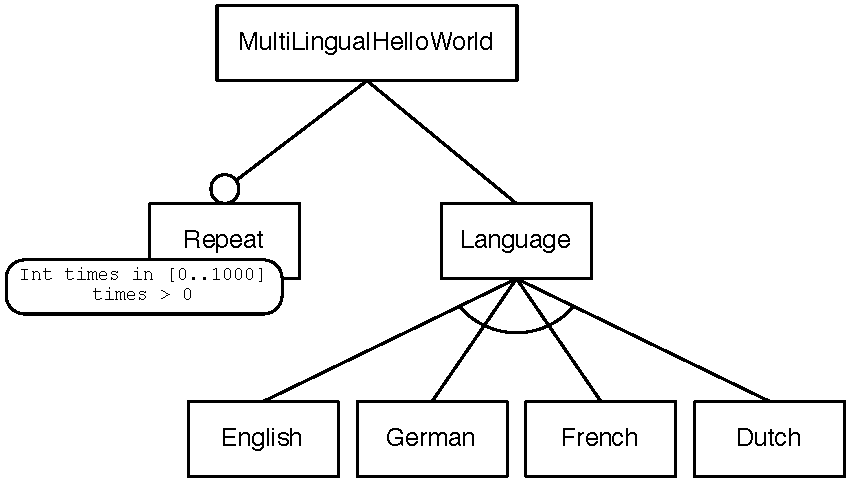
\includegraphics[width=.6\linewidth]{fig/featurediagram}
    \caption{Example feature diagram for a ``Hello World'' software product line}
    \label{fig:feature diagram}
\end{figure}
%
Below we show how the feature model underlying the feature diagram in
Figure~\ref{fig:feature diagram} is encoded in ABS using the textual variability
language \muTVL.
\begin{abscode}
root MultiLingualHelloWorld {
  group allof {
    Language {
      group oneof { English, Dutch, German, French }  
    },
    opt Repeat {
      Int times in [0..1000];
      times > 0; 
    }
  } 
}
extension English {
  Repeat -> (Repeat.times >= 2 && Repeat.times <= 5);
}
\end{abscode}

The ``Hello World'' product line in this example has two main features,
\emph{Language} and \emph{Repeat}, under the root feature and joined with the
\absinline{allof} combinator. The \emph{Language} feature requires one out of
four possible features: \emph{English}, \emph{Dutch}, \emph{French}, or
\emph{German}. The \emph{Repeat} feature is optional, it has no associated
sub-features, and it has an attribute \emph{times} which ranges between 0 and
1000, with an added condition that it must be strictly greater than 0. In this
example an extension for the \emph{English} feature is given. When the
\emph{English} and the \emph{Repeat} features are present, the attribute
\absinline{times} must be between 2 and 5, inclusive.


\subsection{Semantics}

The semantics of \muTVL is given by integer constraints, that is, a feature
model is encoded as a constraint over features and feature attributes. Each
solution for this constraint represents a valid product of the feature model.


\section{Product Selection}
\label{sec:product selection}

ABS allows the developer to name products that are of particular interest, in
order to easily refer to them later when the actual code needs to be generated.
A product definition states which features are to be included in the product and
sets attributes of those features to concrete values.

\subsection{Syntax}
\label{sec:fsl syntax}

Figure~\ref{fig:product selection grammar} shows the grammar of the ABS product selection language. The \NT{Selection}
clause specifies a product by giving it a name, by stating the features and
optional attribute assignments that are included in that product.
% The \NT{FeatureSpec} clause specifies that a given feature is present, and the
% optional \NT{AttributeAssignment} clause is used for specifying the
% attributes, which are assigned concrete values.

% The \NT{InitBlock} clause specifies the
% initialisation block for the given product. This An initialisation block can
% be any core ABS block, but typically will be a simple call to some already
% present \emph{main} method. Initialisation blocks are specified in the product
% selection language to enable product lines with multiple entry points to start
% execution.

\begin{figure}[htp]
    \centering

    \begin{tabular}{rcl}
        \NT{Selection}
        \concrDefn{ \TR{product} \NT{TypeId} \TR{(} \NT{FeatureSpecs} \TR{)} \TR{;} }
        \medskip
        
        \\
        \NT{FeatureSpecs}
        \concrDefn{ \NT{FeatureSpec} \MANYG{\TR{,} \NT{FeatureSpec}} }
        
        \\
        \NT{FeatureSpec}
        \concrDefn{ \fid \OPT{\NT{AttributeAssignments}} }
        \medskip
        
        \\
        \NT{AttributeAssignments}
        \concrDefn{ \TR{\{} \NT{AttributeAssignment} \MANYG{\TR{,} \NT{AttributeAssignment}} \TR{\}} }
        
        \\
        \NT{AttributeAssignment}
        \concrDefn{ \aid \TR{=} \NT{Literal} }
        \medskip
        
        \\      
%       \medskip
        
    \end{tabular}
	\caption{Grammar of the product selection language}
 	\label{fig:product selection grammar}
\end{figure}


\subsection{Example}
A valid product from the example ``Hello World'' product line can be defined as
follows.

\begin{abscode}
product P1 (English);
\end{abscode}
This denotes the inclusion of a single feature, \absinline{English}. Implicitly,
its parent node is also selected. The product \absinline{P2} defined below
includes the features \absinline{Dutch} and \absinline{Repeat}, where
\absinline{Repeat}'s attribute \absinline{times} is initialised to 3. To select
features with attributes, we need to include an assignment of attribute
variables. ABS currently supports boolean and integer feature attributes.
\begin{abscode}
product P2 (Dutch, Repeat{times=3});
\end{abscode}

Below is an \emph{invalid} product definition, that is, one that does not
satisfy the feature model, as the \absinline{Repeat.times} attribute is assigned
a value (2222) outside the valid range defined by the feature model
(\absinline{[0..1000]}). The constraint checker that comes with ABS can evaluate
all product selections with respect to the feature model and warn about invalid
products.
\begin{abscode}
product P3 (English, Repeat{times=2222});
\end{abscode}

\section{Feature Model Reflection}
\label{sec:feat-model-refl}

There is support for limited reflection on the feature model and configured
product in the module \absinline{ABS.Productline}.  The datatype
\absinline{Feature} contains constructors for all feature names.  The function
\absinline{product_features} returns a list of features contained in the
current product, and \absinline{product_name} returns the name of the product,
or the empty string if no product was specified.

The following sample code shows the usage, assuming that product
\absinline{Product} was generated:
\begin{abscode}
module Test;
import * from ABS.Productline;

{
  List<Feature> foo = product_features(); // => Cons(FeatureA, Cons(FeatureC, Nil)) 
  String name = product_name();           // => "Product"
}

productline Test;
features FeatureA, FeatureB, FeatureC;

product Product(FeatureA, FeatureC);
\end{abscode}

% Local Variables:
% TeX-master: "absrefmanual"
% End:

\chapter{Delta Modules}
\label{ch:deltas}

ABS supports the delta-oriented programming model~\cite{SchaeferBBDT10}, an
approach that aids the development of a set of programs simultaneously from a
single code base, following the software product line engineering
approach~\cite{PohlBL05}.
In delta-oriented programming, features defined by a feature model are
associated with code modules that describe modifications to a core program. In
ABS, these modules are called \emph{delta modules}. Hence the implementation of
a software product line in ABS is divided into a \emph{core} and a set of delta
modules.

The core consists of a set of ABS modules containing the classes that implement
a complete software product of the corresponding software product line. Delta
modules (or \emph{deltas} in short) describe how to change the core program to
obtain new products. This includes adding new classes and interfaces, modifying
existing ones, or even removing some classes from the core. Delta modules can
also modify the functional entities of an ABS program, that is, they can add and
modify data types and type synonyms, and add functions.

Deltas are applied to the core program by the ABS compiler front end. The choice
of which delta modules to apply depends on the selection of a set of features,
that is, a particular product of the SPL.
The role of the ABS compiler front end is to translate textual ABS models into
an internal representation and check the models for syntax and semantic errors.
The role of the compiler back end is to generate code for the models targeting
some suitable execution or simulation environment.


\section{Syntax}
\label{delta syntax}
\begin{figure}
    \centering
    \begin{tabular}{rcl}

        \NT{DeltaDecl}
        \concrDefn{ \TR{delta} \NT{TypeId} \OPT{\NT{DeltaParams}} \TRS{;} \OPT{\NT{ModuleAccess}} \MANY{\NT{ModuleModifier}} }
        
        \\
        \NT{ModuleModifier}
        \concrDefn{ \TR{adds} \NT{ClassDecl} }
        \concrCont{ \TR{removes} \TR{class} \NT{TypeName} \TRS{;} }
        \concrCont{ \TR{modifies} \TR{class} \NT{TypeName} }
        \concrNewline{ \OPTG{\TR{adds}\ \NT{TypeId}\ \MANYG{\TRS{,}\ \NT{TypeId}}} \OPTG{\TR{removes}\ \NT{TypeId}\ \MANYG{\TRS{,}\ \NT{TypeId}}} }
        \concrNewline{ \TRS{\{} \MANY{\NT{Modifier}} \TRS{\}} }
        \concrCont{ \TR{adds} \NT{InterfaceDecl} }
        \concrCont{ \TR{removes} \TR{interface} \NT{TypeName} \TRS{;} }
        \concrCont{ \TR{modifies} \TR{interface} \NT{TypeName} \TRS{\{} \MANY{\NT{InterfaceModifier}} \TRS{\}}}
        \concrCont{ \TR{adds} \NT{FunctionDecl} }
        \concrCont{ \TR{adds} \NT{DataTypeDecl} }
        \concrCont{ \TR{modifies} \NT{DataTypeDecl} }
        \concrCont{ \TR{adds} \NT{TypeSynDecl} }
        \concrCont{ \TR{modifies} \NT{TypeSynDecl} }
        \concrCont{ \TR{adds} \NT{Import} }
        \concrCont{ \TR{adds} \NT{Export} }
        \medskip
        \\

        \NT{InterfaceModifier}
        \concrDefn{ \TR{adds} \NT{MethSig} \TRS{;} }
        \concrCont{ \TR{removes} \NT{MethSig} \TRS{;} }
        \medskip
        \\

        \NT{Modifier}
        \concrDefn{ \TR{adds} \NT{FieldDecl}}
        \concrCont{ \TR{removes} \NT{FieldDecl}}
        \concrCont{ \TR{adds} \NT{MethDecl} }
        \concrCont{ \TR{removes} \NT{MethSig} }
        \concrCont{ \TR{modifies} \NT{MethDecl} }
        \medskip
        \\
        
        \NT{DeltaParams}
        \concrDefn{ \TRS{(}\NT{DeltaParam} \MANYG{\TRS{,} \NT{DeltaParams}} \TRS{)}}

        \\
        \NT{DeltaParam}
        \concrDefn{ \NT{Identifier} \MANY{\NT{HasCondition}}}
        \concrCont{ \NT{Type}\ \NT{Identifier} }
        \medskip
        
        \\
        \NT{ModuleAccess}
        \concrDefn{ \TR{uses} \NT{TypeId} \TRS{;}}
        \medskip
        
        \\
        \NT{HasCondition}
        \concrDefn{ \TR{hasField} \NT{FieldDecl} }
        \concrCont{ \TR{hasMethod} \NT{MethSig} }
        \concrCont{ \TR{hasInterface} \NT{TypeId} }
        
    \end{tabular}
    \caption{ABS Grammar: Delta Modules.}
    \label{fig:delta-grammar}
\end{figure}

Figure~\ref{fig:delta-grammar} specifies the ABS syntax related to delta
modeling. The \NT{DeltaDecl} clause specifies the syntax of delta modules,
consisting of an unique identifier, a module access directive, a list of
parameters and a sequence of module modifiers. The \emph{module
access} directive gives the delta access to the namespace of a particular
module. In other words it specifies the ABS module to which the modifications
specified by the delta apply by default. A delta can still apply changes to
several modules by fully qualifying the \NT{TypeName} of module modifiers.

The \NT{ModuleModifier} clause describes the syntax of modifications at the
level of modules. Such a modification can, for example, add a class or interface
declaration, modify an existing class or interface, remove a class or interface,
and also add functions, data types and type synonyms. Class modifications
include the ability to change the interface of a class by adding or removing
items from the class's list of implemented interfaces.
The \NT{InterfaceModifiers} clause describes how to modify existing interface
declarations, either by adding new or removing existing method signatures.

The \NT{Modifier} clause specifies the modifications that can occur within a
class or interface body. These include adding and removing fields and methods,
and modifying methods, which amounts to replacing a method implementation with a
new one, while enabling the original method to be called using the \TR{original}
keyword.
The aim of \absinline{original} is to enable the method being replaced to be
called from the delta module that replaces it. This is implemented by renaming
the original method, and replacing the call to \absinline{original} with a call
to the renamed method. 

A method can be replaced multiple times by applying a succession of deltas. To
call a specific version of such a method, a \emph{targeted} \absinline{original}
call can be used. The target specifies hereby the delta or the core program.

% This gives the user a tighter control over the program's behaviour. It also
% makes the code less flexible because calling \absinline{original} on a
% particular target delta introduces the assumption that the target delta has been
% already applied. Such a dependency could be invalidated for instance by changes
% to the SPL configuration, which dictates which deltas should be applied when
% certain features are selected.

\section{Object-oriented modifiers}
To modify an object-oriented ABS program, delta modules support adding new
classes and removing existing ones. Existing classes can be also modified by
adding new methods and also removing or modifying existing methods.
Deltas can also add new interface declarations, remove existing interface
declarations, and modify interface declarations by adding or removing
operations. Furthermore, deltas can change the interface of a class by adding or
removing interfaces from the class's list of implemented interfaces. Lastly,
delta modules can introduce new fields to classes and remove existing fields.

\subsection{Interfaces}
Deltas can introduce new interface declarations and remove or modify existing
interface declarations. The syntax is illustrated by the following examples.
\begin{abscode}
delta D1;
adds interface MyModule.I { Unit foo(); }

delta D2; 
uses MyModule;
removes interface I;

delta D3;
uses MyModule;
modifies interface I { removes Unit foo(); adds Unit bar(); }
\end{abscode}


\subsection{Classes}
Deltas can introduce new classes and remove existing classes. The syntax is
illustrated by the following examples.
\begin{abscode}
delta D1;
adds class MyModule.DataBase(Map<Filename,File> db) implements DB {...}

delta D2; 
uses MyModule;
removes class Node();
\end{abscode}

The first delta \absinline{D1} above declares a new class \absinline{DataBase} inside the
module \absinline{MyModule}. Delta \absinline{D2} removes the class \absinline{Node} from the same
module.
Specifying to which module such code modifications apply can be done in two
ways. First, as exemplified by delta \absinline{D1}, the class name can be qualified with a module name.
An alternative way is to include a \absinline{uses <Module Name>} clause at the
beginning of the delta module, which \emph{opens} a module so that names don't
need to be qualified. When a delta specifies modifications to a single module,
this method is more concise. When a delta specifies modifications across
multiple modules, it is more convenient to qualify each class modifier with a module
name. Using both methods together is also possible, in which case unqualified
class names will refer to classes defined inside the \emph{used} module.

Deltas can also \emph{modify} existing classes by adding new methods and
removing or modifying methods; by adding or removing fields; and by manipulating
the list of interfaces that the class implements. These operations are illustrated in the
following sections.

\subsection{Methods}
\label{sec:class methods}
Methods can be added, removed or modified from within deltas.
The following example shows a delta module designed to modify the behaviour of
the class \absinline{Greeter} by modifying its \absinline{sayHello} method.
The class is assumed to have been declared in the core program inside the
\absinline{Hello} module.

\begin{abscode}
delta Nl;
uses Hello;
modifies class Greeter {
    modifies String sayHello() {
        return "Hallo wereld";
    }
}
\end{abscode}
%
The above \absinline{Nl} delta module applies its changes to the core ABS module
\absinline{Hello}, as specified by the \absinline{uses} clause. It provides a new
implementation for the method \absinline{sayHello()} in class
\absinline{Greeter} by declaring a so-called method \emph{modifier}. The method modifier
is introduced by the \absinline{modifies} keyword and followed by the method
signature and a block of code providing the method's new implementation.
 
Adding entirely new methods is also supported using the \absinline{adds} keyword
followed by the method signature and its implementation.
Similarly, it is possible to remove methods from classes using
\absinline{removes} followed by the method signature, as shown in the following.
\begin{abscode}
delta D;
modifies class M.Foo {
    adds Int bar() { return 17; }
    removes Unit moo();
}
\end{abscode}

% \subsubsection{Delta parameters}
% \label{sec:delta parameters}
% Deltas take an optional list of parameters. These are used to pass on
% configuration information defined in the product selection (cf.
% Section~\ref{sec:product selection}) down to the implementation level. Product
% declarations assign a boolean value to each feature (true if selected, false
% otherwise), and a value to each feature attribute (of features that are
% selected). Delta parameters must be immutable objects, such as booleans,
% integers, or strings.
% 
% In the example below, any occurrence of the integer variable \absinline{times}
% inside the delta module is replaced with the concrete value of the feature
% attribute \absinline{Repeat.times} (from the ``Hello World'' example in
% Section~\ref{sec:feature model}) upon delta application. The connection between
% feature attributes and delta parameters is defined in the SPL configuration, 
% which is described in Section~\ref{ch:spl configuration}.
% \begin{abscode}
% delta Rpt (Int times);
% modifies class Hello.Greeter {
%     modifies String sayHello() {
%         String result = "";
%         Int i = 0;
%         while (i < times) {
%             String orig = original();
%             result = result + " " + orig;
%             i = i + 1;
%         }
%         return result;
%     }
% }
% \end{abscode}
% For example, when building the product ``\absinline{P2(Dutch, Repeat\{times=3\})}'',
% the \absinline{times} variable inside the \absinline{while} loops' predicate
% is replaced with the integer constant ``\absinline{3}''.
% 
% The boolean values of features can be accessed in similar fashion, as shown in
% the example below. Here, a delta adds three fields to class \absinline{C}, which
% are assigned boolean constants that reflect whether the features to which they
% are connected are selected or not. In this way, one can easily write code that
% reflects on the feature configuration.
% \begin{abscode}
% delta D (Bool a, Bool b, Bool c);
% modifies class C {
%     adds Bool featureA = a;
%     adds Bool featureB = b;
%     adds Bool featureC = c;
% }
% \end{abscode}

\subsubsection{Calling \absinline{original}}
%A notable artifact in the above example is the statement \absinline{String orig = original()}. 
Calling \absinline{original} from within a method modifier body makes it
possible to access the method's previous behaviour, that is, the behaviour
implemented in the previously applied delta or in the core. This is similar to
calling \absinline{super} to access the superclass behaviour of a method in a language
with class inheritance such as Java. An \absinline{original} call has to supply a list
of arguments that conforms with the original method's list of formal parameters.

\subsubsection{Targeted \absinline{original} calls}
Original calls can be targeted towards a given delta by prefixing the call with
the name of the delta, or towards the core ABS code by using the keyword
\absinline{core}:
\begin{abscode}
core.original(params);
Delta.original(params);
\end{abscode}

Regular (untargeted) original calls invoke the method behaviour defined by the previously applied delta.
% current at the time before application of the delta where the call is issued. 
For example, if a method \absinline{m} is defined in the core, and then a set of deltas
\absinline{D1..D3}, which each modify \absinline{m}, are applied in sequence,
then calling \absinline{original} from within \absinline{m}'s modifier in
\absinline{D3} will run the version of \absinline{m} defined in \absinline{D2}.
With a targeted call, one can access any version of \absinline{m}, that is, the
versions defined in \absinline{D2}, \absinline{D1} and in the core.

This allows a tighter control of which code is actually executed
when calling \absinline{original}. As the order of delta application is often
not uniquely defined, it is not always determinable which behaviour will be invoked upon
calling \absinline{original}. With a targeted original call, the user can
specify exactly which code to execute and even invoke multiple versions of a
method. This, of course, implies that the target delta has been applied already;
otherwise the compiler will indicate an error.

\begin{abscode}
module M;
class C {
    String m(String s) { return(s) };
}
delta D1;
modifies M.C {
    modifies String m(String s) { return prefix + original(s); }
}
delta D2;
modifies M.C {
    modifies String m(String s) { return original(s) + suffix; }
}
delta Resolve;
modifies M.C {
    modifies String m(String s) { return prefix + core.original(s) + suffix; }
}
\end{abscode}

Consider the above example. \absinline{D1} and \absinline{D2} both modify method \absinline{m} in
different, non-compatible ways. We say that these two deltas are in conflict.
Assume that \absinline{D1} and \absinline{D2} can be applied in any order, and that delta
\absinline{Resolve} has to be applied after \absinline{D1} and \absinline{D2}. By calling
\absinline{original} from within \absinline{Resolve}, we cannot be sure which version of
\absinline{m} will actually be invoked: this depends on whether \absinline{D1} or \absinline{D2}
has been applied last. By targeting the original call towards a specific delta,
we can control the behaviour precisely, and resolve the conflict in a meaningful
way.

Targeted original calls were required for the implementation of the delta
modelling workflow (DMW)~\cite{Helvensteijn12,HelvensteijnMW12}, which is
described in more detail in Deliverable 5.3~\cite{d5.3}. The DMW describes a
process of applying delta modelling to obtain a model of a software product line
that is globally unambiguous and complete. A focus of DMW is the systematic
reconciliation of conflicting feature functionality.


\subsection{Class interfaces}
A delta module can change the list of interfaces that a class implements.
Adding or dropping interfaces from that list is achieved using the familiar
\absinline{removes} and \absinline{adds} keywords.

The following example shows a core ABS program defining a \absinline{Logger}
class that implements the \absinline{Output} interface. It further declares a
delta module that modifies the \absinline{Logger} class such that it
implements a different interface. This new  \absinline{IO} interface is 
introduced in the same delta.
%
\begin{abscode}
module M;
interface Input { String read(); }
interface Output { Unit write(String s); }
class Logger implements Output {
    Unit write(String s) {...}
}

delta IO;
adds interface IO extends Input, Output {}
modifies class Logger adds IO removes Output {
    adds String read() {...}
}
\end{abscode}

\subsection{Fields}
In addition to modifying object behaviour, ABS allows adding or removing fields.
New fields are introduced by the \absinline{adds} keyword followed by the
field's type, name, and an optional value assignment. Similarly, fields can be
removed using the \absinline{removes} keyword. The following example demonstrates this.
\begin{abscode}
delta D;
modifies class M.Foo {
    adds List<Item> items;
    adds Int itemsCount = items.size();
    removes String name;
}
\end{abscode}



\section{Functional modifiers}
Functional program elements can also be modified from within deltas.
ABS supports the addition of functions, data types and type synonyms,
and the modification of data types and type synonyms.  Qualifying
functional elements with the module name is currently unsupported,
therefore when adding functional elements, a \absinline{uses} clause has
to be specified.

\subsection{Functions}
Example of adding a function.

\begin{abscode}
delta MyDelta;
uses MyModule;
adds def Int min(Int a, Int b) = case a < b { True => a; False => b; };
\end{abscode}

\subsection{Data types}
\label{sec:data types}
Example of adding a data type.
\begin{abscode}
adds data Schedule = Schedule(
    String schedname,
    List<Item> items,
    Int sched,
    Deadline dline) | NoSchedule;
\end{abscode}

\noindent
Example of modifying a data type.
\begin{abscode}
modifies data Schedule = Schedule(
    String schedname,
    List<Item> items,
    Int sched,
    Deadline dline) | NoSchedule(String reason);
\end{abscode}
When modifying a datatype, the given constructors supersede the previous
list of constructors.

\subsection{Type synonyms}
Example of adding a type synonym.
\begin{abscode}
adds type ClientId = Int;
\end{abscode}

\noindent
Example of modifying a type synonym.
\begin{abscode}
modifies type ClientId = String;
\end{abscode}


\section{Module modifiers}
Deltas support, to some extent, modifications to ABS's module system.

\subsection{Imports and Exports}
The addition of (qualified and unqualified) \absinline{import}s and \absinline{export}s to modules
(cf. Chapter~\ref{sec:modules}) is supported, as shown in the following examples.

\begin{abscode}
delta D1;
uses Drinks;
adds export Drink, Milk;

delta D2;
uses Bar;
adds export *;
adds import Drinks.Milk;

delta D3;
uses MyModule;
adds import * from Bar;
\end{abscode}
%
The \absinline{adds import} and \absinline{adds export} directives apply to the
module defined by the \absinline{uses} statement.


\section{Unsupported modifications}

While delta modelling supports a broad range of ways to modify an ABS model, not
all ABS program entities are modifiable. These unsupported modifications are
listed here for completeness. While these modifications could be easily
specified and implemented, we opted not to overload the language with features
that have not been regarded as necessary in practice.
 
\begin{description}
    \item[Class parameters and init block] Deltas currently do not support the 
    modification of class parameter lists or class init blocks.

  \item[Functional program elements] Deltas currently only support
    adding functions, and adding and modifying data types and type
    synonyms. Removal is not supported.

    \item[Modules] Deltas currently do not support adding new modules or removing modules.
    
    \item[Imports and Exports]While deltas do support the addition of \absinline{import} and
    \absinline{export} statements to modules, they do not support their modification or removal.
    
    \item[Main block] Deltas currently do not support the modification of the program's main block.

\end{description}

% Local Variables:
% TeX-master: "absrefmanual"
% End:

\chapter{Software Product Line Configuration \\and Product Generation}
\label{ch:spl configuration}

\section{Software Product Line Configuration}
\label{sec:spl configuration}

The ABS configuration language links feature models, which describe the
structure of a SPL (Chapter~\ref{ch:feature modelling}), to delta modules
(Chapter~\ref{ch:deltas}), which implement behaviour. This link is illustrated
in Fig.~\ref{fig:variability overview}. The configuration defines, for each
selection of features satisfied by the product selection, which delta modules should
be applied to the core. Furthermore, it guides the code generation by ordering
the application of the delta modules.

\begin{figure}
    \centering
    \tikzstyle{box3} = [draw=gray!50, fill=gray!15, thick, rounded corners=1pt]
\tikzstyle{process} = [fill=yellow!90!black, thick, rounded corners=6pt]
\tikzstyle{structure} = [box3, fill=blue!30]
\tikzstyle{behaviour} = [structure, fill=red!40, minimum width=4em]
\tikzstyle{line} =[line width=2\unitlength, black!60, >=latex]
\tikzstyle{thickarrow} =[->,line width=14\unitlength, draw=green!70!black, fill=green!70!black, >=triangle 90 cap]

\begin{tikzpicture}
    [xscale=4.5, yscale=-2.2,
    sm/.style={font=\small,auto}]
    \node[structure] at (1,1) (fm) {Feature Model};
    \node[structure] at (1,3) (ps) {Product Selection};
    \node[process] at (2,2) (conf) {Configuration};
    
    \draw[line,->] (fm) to node[sm] {} (ps);
    \draw[line,dotted,->] (conf) to node[sm,above] {ensures satisfaction} ($(fm)!.5!(ps)$);

    \node[box3,matrix,row sep=2\unitlength,label=above:Modules] at (3,1) (code) {
        \node[behaviour] {Core}; \\ 
        \node[behaviour] {Deltas}; \\
    };

    \node[behaviour] at (3,3) (prod) {Software Product};
    \draw[line] (fm) to (code);
    \draw[line,->,dotted] (conf) to node[sm,sloped,midway,above] {associates} ($(fm)!.5!(code)$);
    \draw[line,dotted,->] (conf) to node[sm] {guides} ($($(code)!.5!(prod)$)!1.5\unitlength!90:(prod)$);

    \draw[thickarrow] (code) to node[sloped,midway,rotate=180,white] {Code Generation} (prod);
\end{tikzpicture}

    \caption{Variability modelling framework of ABS
%   \JP{to Radu: I find hard to explain how a configuration ensures satisfaction. And maybe we should swap FM and PS?}
    }
    \label{fig:variability overview}
\end{figure}

Features and delta modules are associated through \emph{application conditions},
which are logical expressions over the set of features and attributes in a
feature model. The collection of applicable delta modules is given by the
application conditions that are true for a particular feature and attribute
selection. By not associating the delta modules directly with features, a degree
of flexibility is obtained.

\subsection{Syntax}
\label{spl configuration syntax}

The SPL \NT{Configuration} clause specifies the name of the product
line, the set of \NT{Features} it provides, and the set of delta modules used to
implement those features. The feature names are included so that certain simple
self-consistency checks can be performed. The \NT{DeltaClause} is used to
specify each delta module, linking it to the feature model.

\begin{abssyntax}
    \NT{Configuration}
    \concrDefn{ \TR{productline} \NT{TypeId} \TR{;} \NT{Features} \TR{;} \NT{DeltaClauses} }
    \\
    \NT{Features}
    \concrDefn{\TR{features} \fid \MANYG{\TR{,} \fid} }
    \\
    \NT{DeltaClauses}
    \concrDefn{ \MANY{\NT{DeltaClause}} }
    \\
    \NT{DeltaClause}
    \concrDefn{ \TR{delta} \NT{DeltaSpec} \OPT{\NT{AfterCondition}} \OPT{\NT{ApplicationCondition}} \TR{;} }
    \medskip
    \\
    \NT{DeltaSpec}
    \concrDefn{ \NT{TypeName} \OPT{\TR{(} \NT{DeltaParams} \TR{)}} }
    \\
    \NT{DeltaParams}
    \concrDefn{ \NT{DeltaParam} \MANYG{\TR{,} \NT{DeltaParam}} }
    \\
    \NT{DeltaParam}
    \concrDefn{\fid  $|$ \fid.\aid}
%    \concrDefn{\fid  $|$ \fid.\aid  $|$ \NT{DataExp}}
    \\
    \NT{AfterClause}
    \concrDefn{ \TR{after} \NT{TypeName} \MANYG{\TR{,} \NT{TypeName}} }
    \\
    \NT{WhenClause}
    \concrDefn{ \TR{when} \NT{AppCond} }
    \\
    \NT{AppCond}
    \concrDefn{ \NT{AppCond} \TRS{\&\&} \NT{AppCond} }
    \concrCont{ \NT{AppCond} \TRS{||} \NT{AppCond} } 
    \concrCont{ \TR{\sim} \NT{AppCond} } 
    \concrCont{ \TR{(} \NT{AppCond} \TR{)} } 
    \concrCont{ \fid } 
\end{abssyntax}
%
Each delta clause has a \NT{DeltaSpec}, specifying the name of a delta module
name and, optionally, a list of parameters; an \NT{AfterClause}, specifying the
delta modules that the current delta must be applied after; and an application
condition \NT{AppCond}, specifying an arbitrary predicate over the feature and
attribute names in the feature model that describes when the given delta module
is applied.

\subsection{Delta parameters} \label{sec:delta parameters}
A delta clause takes an optional list of \NT{DeltaParams}, which are either
features or fully qualified feature attributes. When a particular
product of the product line is selected (as described in
Section~\ref{sec:product selection}), the value \absinline{true} is assigned to each of
its features and a value is assigned to each of its features' attributes.
These values can be used inside the delta module if the corresponding delta clause
specifies the feature or feature attribute as one of its parameters.


\subsection{Application Conditions}
\label{sec:application conditions}
The configuration is used to specify conditions under which a delta module
should be applied to the core. Such application conditions are propositional
formulas over the set of features and attributes defined by the feature model.
They can be in terms of the presence and absence of features and feature
combinations, as well as attributes of features and integer and boolean
constants. When the propositional formula holds for a given product, the delta
module is applicable. Application conditions are introduced by the \absinline{when}
keyword, as shown in the examples below.
\begin{absexample}
delta D when A or B and ~C;
delta LargeCache when Mem.size > 1024;
\end{absexample}

\subsection{Application Order of Delta Modules}
\label{sec:delta ordering}
For each delta module, the configuration establishes a partial ordering relation
with respect to other deltas by using the \absinline{after} keyword. The partial
order states which delta modules, when applicable, should be applied before the
given delta module.


\subsection{Configuration Example}
A configuration specifies the name of the product line, the set of
features it provides, and the set of delta modules used to implement those
features.

\begin{absexample}
productline MultiLingualHelloWorld;
    features English, German, Dutch, Repeat;
    delta De when German;
    delta Nl when Dutch;
    delta Fr when French;
    delta Rpt(Repeat.times) after De, Nl, Fr when Repeat;
\end{absexample}

The example above first names the set of features from the feature model (cf.
Section~\ref{sec:feature model example}) used to configure this product line.
The \absinline{delta} clauses link each delta module to the feature model
through an application condition (\absinline{when} clause); in this case, a
delta module is applied simply when the specified feature is selected (e.g.
``\absinline{De when German}''). There is no delta module corresponding to the
feature \absinline{English}, as the core module provides support for the English
language by default. In addition, \absinline{Rpt} has to be applied
\absinline{after} \absinline{De}, \absinline{Nl} and \absinline{Fr}.
The \absinline{Rpt} delta has a parameter \absinline{Repeat.times}, the
\absinline{times} attribute of the feature \absinline{Repeat}; its value
(defined by product selection, see Section~\ref{sec:product selection}) is
propagated to the \absinline{Rpt} delta as described in Section~\ref{sec:delta parameters}.


\section{Product Generation}
\label{sec:product generation}

The process of generating a software product from a given software product line
relies on the full ABS specification of an SPL, that is, a feature model with a
set of product declarations (Chapter~\ref{ch:feature modelling}), a set of delta
modules (Chapter~\ref{ch:deltas}), and a configuration that connects the two
(Section~\ref{sec:spl configuration} above).
To generate a particular product, this has to be selected either using the
Eclipse IDE (cf. Figure~\ref{fig:eclipse product generation}), or given as an argument when invoking the compiler
on the command line. For example:

\begin{cmdline}
generateJava -product=P2 Hello.abs
\end{cmdline}

\begin{figure}[htp]
	\centering
	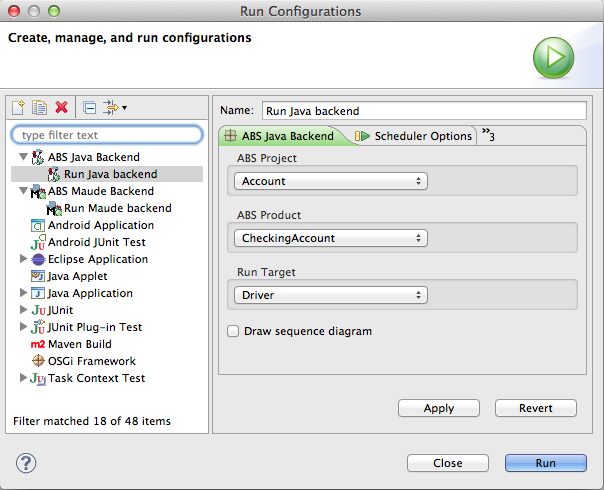
\includegraphics[width=.9\linewidth]{fig/eclipse-product-generation}
	\caption{SPL product generation using the Eclipse IDE}
 	\label{fig:eclipse product generation}
\end{figure}

\subsection{Example}

For example, selecting the product \absinline{P2} of the ``Hello world'' product line
triggers the compiler to execute through the following steps.

\begin{enumerate}
    \item Check if the product is valid with respect to the feature model. 
    In this case the product \absinline{P2} is valid.

    \item Find all applicable delta modules. In this case the deltas modules
    with an application condition that holds are \absinline{Nl} and
    \absinline{Rpt(3)}.
  
    \item Linearise the application order of delta modules. The restriction here
    is over the delta module \absinline{Rpt}, which has to follow any of the
    language deltas.
  
    \item Apply the deltas sequentially. First, the \absinline{Nl} delta is applied
    to the Core ABS program. Then the \absinline{Rpt(3)} delta is applied to
    the result of the previous application.
\end{enumerate}

\noindent The result is a core ABS program.

\chapter{Annotations}
ABS supports \emph{Annotations} to enrich an ABS model with additional information, for example, to realize pluggable type systems.
Annotations can appear before any declaration and type usage in ABS programs (which is not given in the grammar definitions, to improve readability).

\begin{abssyntax}
\NT{Annotation} \defn \TRS{[}\ \OPTG{\NT{TypeName}\ \TRS{:}}\ \NT{PureExp}\ \TRS{]}
\end{abssyntax}

\begin{absexample}
[LocationType:Near] Peer p;
[Far] Network n;
List<[Near] Peer> peers = Nil;
\end{absexample}

\section{Type Annotations}
ABS has a predefined meta-annotation \absinline{TypeAnnotation} to declare
annotations to be \emph{Type Annotations}.
Data types that are annotated with that annotation are specially treated by the
ABS compiler to support an easier implementation of pluggable type systems.

\begin{absexample}
[TypeAnnotation]
data LocationType = Far | Near | Somewhere | Infer;
\end{absexample}

\chapter{Models}
\label{sec:model}
A \emph{model} in ABS represents a type-closed set of \emph{modules}.
A module defines a set of declarations and an optional \emph{main block}.
Modules reside in \emph{compilation units}, which are typically represented by files ending with \texttt{.abs}.
A model is thus set of compilation units.

\begin{abssyntax}
\NT{Model}           \defn \MANY{\NT{CompilationUnit}}\\
\NT{CompilationUnit} \defn \MANY{\NT{ModuleDecl}} \NT{FeatureModel}
\end{abssyntax}



\bibliographystyle{plain}
\bibliography{bibli}








\appendix
\chapter{ABS Standard Library}\label{ch:absstdlib}
%\lstinputlisting[style=abs]{code/abslang.abs}


\begin{abscode}
module ABS.StdLib;
export *;
export Cost;
import Cost from ABS.DC;
\end{abscode}

\section{Built-in Datatypes}

\begin{abscode}
data Unit = Unit;               // builtin  
data String;                    // builtin  
data Int;                       // builtin
data Rat;                       // builtin
data Bool = True | False;       // builtin
data Fut<A>;                    // builtin
data Location;                  // (For Component model) //
\end{abscode}

\section{Boolean and Numeric Functions}

\begin{abscode}
def Bool and(Bool a, Bool b) = a && b;
def Bool not(Bool a) = ~a;

def Rat max(Rat a, Rat b) = if a > b then a else b;
def Rat min(Rat a, Rat b) = if a < b then a else b;
    
def Rat abs(Rat x) = if x > 0 then x else -x;
/**
 * Returns a random number between 0 (inclusive) and below (exclusive).
 */
def Int random(Int below) = builtin;

/**
 * Truncates a towards zero.
 */
def Int truncate(Rat a) = builtin;
\end{abscode}

\section{Optionals and Tuples}

\begin{abscode}
data Maybe<A> = Nothing | Just(A fromJust);

def Bool isJust<A>(Maybe<A> a) = 
    case a { Just(j) => True; Nothing => False; };

data Either<A, B> = Left(A left) | Right(B right);

def Bool isLeft<A,B>(Either<A, B> val) = 
    case val { Left(x) => True; _ => False; };
    
def Bool isRight<A,B>(Either<A, B> val) = ~isLeft(val);


data Pair<A, B> = Pair(A fst, B snd); 

data Triple<A, B, C> = Triple(A fstT, B sndT, C trd); 
\end{abscode}

\section{Sets}

\begin{abscode}
// Sets are currently implemented as sorted lists (any implementation
// must yield the same structure regardless of insertion order so that
// set equality via == is preserved).  Using the Insert_ constructor
// directly is strongly discouraged.
data Set<A> = EmptySet | Insert(A, Set<A>);

// set constructor helper
def Set<A> set<A>(List<A> l) = 
    case l { 
       Nil => EmptySet; 
       Cons(x,xs) => insertElement(set(xs), x);
    };

/**
 * Returns True if set 'ss' contains element 'e', False otherwise.
 */
def Bool contains<A>(Set<A> ss, A e) =
  case ss {
    EmptySet => False ;
    Insert(e, _) => True;
    Insert(x, xs) => if x > e then False else contains(xs, e);
  };
  
/**
 * Returns True if set 'xs' is empty, False  otherwise.
 */
def Bool emptySet<A>(Set<A> xs) = (xs == EmptySet); 

/**
 * Returns the size of set 'xs'.
 */
def Int size<A>(Set<A> xs) = 
   case xs {
      EmptySet => 0 ; 
      Insert(s, ss) => 1 + size(ss); 
   };

def Set<A> union<A>(Set<A> set1, Set<A> set2) =
   case set1 {
      EmptySet => set2;
      Insert(e1, ss1) =>  case set2 {
          EmptySet => set1;
          Insert(e1, ss2) => Insert(e1, union(ss1, ss2));
          Insert(e2, ss2) =>
            if e1 < e2
            then Insert(e1, union(ss1, set2))
            else Insert(e2, union(set1, ss2));
      };
   }; 

/**
 * Returns a set with all elements of set 'xs' plus element 'e'.
 * Returns 'xs' if 'xs' already contains 'e'.
 */
def Set<A> insertElement<A>(Set<A> xs, A e) =
  case xs {
      EmptySet => Insert(e, EmptySet);
      Insert(e, _) => xs;
      Insert(x, ss) => if e < x then Insert(e, xs) else Insert(x, insertElement(ss, e));
  };


/**
 * Returns a set with all elements of set 'xs' except element 'e'.
 */
def Set<A> remove<A>(Set<A> xs, A e) = 
  case xs {
     EmptySet => EmptySet ;
     Insert(e, ss) => ss;
     Insert(x, ss) => if e < x then xs else Insert(x, remove(ss, e));
  };

/**
 * Returns one (arbitrary) element from a set.
 * To iterate over a set, take one element and remove it from the set.
 * Repeat until set is empty.
 */
def A take<A>(Set<A> ss) =
  case ss {
    Insert(e, _) => e;
  };

// checks whether the input set has more elements to be iterated.
def Bool hasNext<A>(Set<A> s) = ~ emptySet(s); 

// Partial function to iterate over a set.
def Pair<Set<A>,A> next<A>(Set<A> s) = 
   case s { 
      Insert(e, set2) => Pair(set2,e); 
   };
\end{abscode}

\section{Lists}

\begin{abscode}
// Lists
data List<A> = Nil | Cons(A head, List<A> tail);

def List<A> list<A>(List<A> l) = l; // list constructor helper

/**
 * Returns the length of list 'list'.
 */
def Int length<A>(List<A> list) = 
   case list { 
      Nil => 0 ; 
      Cons(p, l) => 1 + length(l) ; 
   };

/**
 * Returns True if list 'list' is empty, False otherwise.
 */
def Bool isEmpty<A>(List<A> list) = list == Nil;

/**
 * Returns element 'n' of list 'list'.
 */
def A nth<A>(List<A> list, Int n) = 
  case n { 
    0 => head(list) ; 
    _ => nth(tail(list), n-1); 
  };
  
/**
 * Returns a list where all occurrences of a have been removed
 */
def List<A> without<A>(List<A> list, A a) =
  case list {
     Nil => Nil;
     Cons(a, tail) => without(tail,a);
     Cons(x, tail) => Cons(x, without(tail,a));
  };  
  
/**
 * Returns a list containing all elements of list 'list1'
 * followed by all elements of list 'list2'.
 */
def List<A> concatenate<A>(List<A> list1, List<A> list2) =
  case list1 { 
    Nil => list2 ; 
    Cons(head, tail) =>  Cons(head, concatenate(tail, list2)); 
  };
  
/**
 * Returns a list containing all elements of list 'list' followed by 'p'.
 */
def List<A> appendright<A>(List<A> list, A p) = 
    concatenate(list, Cons(p, Nil));

/**
 * Returns a list containing all elements of 'list' in reverse order.
 */
def List<A> reverse<A>(List<A> list) =
  case list { 
     Cons(hd, tl) => appendright(reverse(tl), hd); 
     Nil => Nil; 
  };
  
/**
 * Returns a list of length 'n' containing 'p' n times.
 */
def List<A> copy<A>(A p, Int n) = 
   case n { 0 => Nil; m => Cons(p,copy(p,m-1)); };
\end{abscode}

\section{Maps}

\begin{abscode}
// Maps
data Map<A, B> = EmptyMap | InsertAssoc(Pair<A, B>, Map<A, B>);
 // map constructor helper (does not preserve injectivity)
def Map<A, B> map<A, B>(List<Pair<A, B>> l) =
  case l { 
     Nil => EmptyMap; 
     Cons(hd, tl) => InsertAssoc(hd, map(tl)); 
  };
  
  
def Map<A, B> removeKey<A, B>(Map<A, B> map, A key) = // remove from the map
  case map {
  	EmptyMap => map;
    InsertAssoc(Pair(key, _), m) => m;
    InsertAssoc(pair, tail) => InsertAssoc(pair, removeKey(tail, key));
  };
    

def List<B> values<A, B>(Map<A, B> map) =
  case map {
    EmptyMap => Nil ;
    InsertAssoc(Pair(_, elem), tail) => Cons(elem, values(tail)) ;
  };

/**
 * Returns a set containing all keys of map 'map'.
 */
def Set<A> keys<A, B>(Map<A, B> map) =
  case map { 
    EmptyMap => EmptySet ;
    InsertAssoc(Pair(a, _), tail) => Insert(a, keys(tail)); 
  };
    
/**
 * Returns the value associated with key 'k' in map 'ms', or 'Nothing'.
 */
def Maybe<B> lookup<A, B>(Map<A, B> ms, A k) = // retrieve from the map
  case ms {
     InsertAssoc(Pair(k, y), _) => Just(y);
     InsertAssoc(_, tm) => lookup(tm, k);
     EmptyMap => Nothing;
  };

/**
 * Compatibility stub for bug 342. DEPRECATED!
 */
def Maybe<B> lookupMaybe<A, B>(Map<A, B> ms, A k) = lookup(ms, k);

/**
 * Returns the value associated with key 'k' in map 'ms',
 * or fails if not present.
 */
def B lookupUnsafe<A, B>(Map<A, B> ms, A k) = // retrieve from the map
  fromJust(lookup(ms,k));
  
/**
 * Returns the value associated with key 'k' in map 'ms', or the value 'd'
 * if 'k' has no entry in 'ms'.
 */
def B lookupDefault<A, B>(Map<A, B> ms, A k, B d) = // retrieve from the map
  case ms {
     InsertAssoc(Pair(k, y), \_) => y;
     InsertAssoc(\_, tm) => lookupDefault(tm, k, d);
     EmptyMap => d;
  };

/**
 * Returns a map with all entries of 'map' plus an entry 'p',
 * which might override but not remove another entry with the same key.
 */
def Map<A, B> insert<A, B>(Map<A, B> map, Pair<A, B> p) = InsertAssoc(p, map);

/**
 * Returns a map with all entries of 'ms' plus an entry mapping 'k' to 'v',
 * minus the first entry already mapping 'k' to a value.
 */  
def Map<A, B> put<A, B>(Map<A, B> ms, A k, B v) =
  case ms {
    EmptyMap => InsertAssoc(Pair(k, v),EmptyMap);
    InsertAssoc(Pair(k, \_), ts) => InsertAssoc(Pair(k, v), ts);
    InsertAssoc(p, ts) => InsertAssoc(p, put(ts, k, v));
  };
\end{abscode}

\section{String Functions}

\begin{abscode}
/**
 * Returns a string with the base-10 textual representation of 'n'.
 */
def String intToString(Int n) =
  case n < 0 {
    True => "-" + intToStringPos(-n);
    False => intToStringPos(n);
  };

def String intToStringPos(Int n) =
  let (Int div) = (n / 10) in
  let (Int res) = (n % 10) in
  case n {
    0 => "0"; 1 => "1"; 2 => "2"; 3 => "3"; 4 => "4";
    5 => "5"; 6 => "6"; 7 => "7"; 8 => "8"; 9 => "9";
    \_ => intToStringPos(div) + intToStringPos(res);
  };

/**
 * Returns a substring of string str of the given length starting from start (inclusive)
 * Where the first character has index 0
 * 
 * Example:
 *    substr("abcde",1,3) => "bcd"
 *     
 */
def String substr(String str, Int start, Int length) = builtin;

/**
 * Returns the length of the given string
 */
def Int strlen(String str) = builtin;


/**
 * Returns a string representation for t.
 */
def String toString<T>(T t) = builtin;
\end{abscode}

\section{Times and Durations}

\begin{abscode}
// Time and Duration datatypes.

// Time can be an integer value or InfTime.  Duration is aways an
// integer.
// 
// Durations can be added and subtracted from Times, and compared to
// each other.  Times can be compared to each other.
data Time = Time(Rat timeValue);
def Int currentms() = builtin;
def Time now() = Time(currentms());

// use this like so:
//   Time t = now(); await timeDifference(now(), t) > 5;
def Rat timeDifference(Time t1, Time t2) =
  abs(timeValue(t2) - timeValue(t1));
def Bool timeLessThan(Time t1, Time t2) =
  timeValue(t1) < timeValue(t2);

data Duration = Duration(Rat durationValue) | InfDuration;
def Bool isDurationInfinite(Duration d) = 
  case d { Duration(\_) => False; InfDuration => True; };

def Time addDuration(Time t, Duration d) =
  Time(timeValue(t) + durationValue(d));

def Time subtractDuration(Time t, Duration d) =
  Time(timeValue(t) - durationValue(d));

def Bool durationLessThan(Duration d1, Duration d2) =
  case d1 {
      Duration(v1) => case d2 {
          Duration(v2) => v1 < v2; 
          InfDuration => False; };
      // If d1 and d2 are infinite, < is not antisymmetric ...
      InfDuration => False;
  };

// negative if no (i.e. infinite) deadline
def Rat lowlevelDeadline() = builtin;
def Duration deadline() = 
  case lowlevelDeadline() < 0 {
      True => InfDuration;
      False => Duration(lowlevelDeadline());
  };

def Duration subtractFromDuration(Duration d, Rat v) =
  case d {
      InfDuration => InfDuration;
      Duration(x) => Duration(max(x - v, 0));
  };

// Annotation data type to express deadlines:
// [Deadline: Duration(5)] o!m();
type Deadline = Duration;
type Critical = Bool;

\end{abscode}

\section{Annotations}

\begin{abscode}
/**
 * Annotation data type to define the type of annotations
 * currently only TypeAnnotation exists
 */
data Annotation = TypeAnnotation; 
 
[TypeAnnotation]
data LocationType = Far | Near | Somewhere | Infer;
 
/**
 * Can be used to annotated classes and to ensure that
 * classes are always instantiated in the right way.
 * I.e. classes annotated with [COG] must be created by using
 * new, class annotated with [Plain] must be created by using
 * new local
 */
data ClassKindAnnotation = COG | Plain;

/**
 * Declare local variables to be final
 */
data FinalAnnotation = Final;

/**
 * Declare methods to be atomic, i.e., such methods must not
 * contain scheduling code and also no .get
 */ 
data AtomicityAnnotation = Atomic;

// functional break point
def A watch<A>(A val) = builtin;
def A watchEx<A, B>(A val, B info) = builtin;
\end{abscode}

\section{Custom Schedulers}

\begin{abscode}
/**
 * Custom schedulers
 */
module ABS.Scheduler;
export *;
import * from ABS.StdLib;

data Scheduler;

// The Process datatype, passed to custom schedulers.
// 
// Pid, Process have no constructor, so this datastructure can't be generated within Abs
data Pid;
data Process;

def String method(Process p) = builtin;
def Time arrival(Process p) = builtin;
def Duration cost(Process p) = builtin;
def Duration procDeadline(Process p) = builtin;
def Time start(Process p) = builtin;
def Time finish(Process p) = builtin;
def Bool crit(Process p) = builtin;
def Int value(Process p) = builtin;

def Process defaultscheduler(List<Process> queue) = head(queue);

def Process randomscheduler(List<Process> queue) = nth(queue, random(length(queue)));
\end{abscode}

\section{The Foreign Language Interface}

\begin{abscode}
/**
 * Foreign language interface (FLI) definitions
 */
module ABS.FLI;
export *;

data FLIAnnotation = Foreign;
\end{abscode}

\section{Deployment Modeling}

\begin{abscode}
/** 
 * Deployment components
 * Used to model aspects of hardware configurations and deployment.
 */
module ABS.DC;
export DC, DeploymentComponent, thisDC, Cost, DCData, InfCPU, CPU, capacity, CogLocation;
import * from ABS.StdLib;

data DCData = InfCPU
            | CPU(Int capacity);

// Sums things up in percents (thus the * 100, which makes us not lose
// precision.)
def Rat sumDivsN(List<Int> consumeds, List<Int> totals, Int n) =
  if (n==0 || isEmpty(consumeds) || isEmpty(totals))
  then 0
  else (head(consumeds) * 100 / head(totals)) + sumDivsN(tail(consumeds), tail(totals), n-1);

def Rat averageDivsN(List<Int> consumeds, List<Int> totals, Int length) =
  let (Int mins) = min(length, min(length(consumeds), length(totals)))
  in sumDivsN(consumeds, totals, mins) / mins;

interface DeploymentComponent {
    [Atomic] DCData available();
    [Atomic] Rat load(Int periods);
    [Atomic] DCData total();
    Unit transfer(DeploymentComponent target, Int amount);
    Unit decrementResources(Int amount);
    Unit incrementResources(Int amount);
}

class DeploymentComponent (String description, DCData cpu)
implements DeploymentComponent {
    Time creationTime = now();
    List<Int> history = Nil;      // updated by Maude interpreter
    List<Int> totalhistory = Nil; // ditto; will stay empty for InfCPU case
    Int internalState = 0;
    Bool initialized = False;
    DCData nextcpu = cpu;
    {
        this.initialized = True;
    }
    [Atomic] DCData available() {
        return if (cpu == InfCPU) then InfCPU else CPU(capacity(cpu) - internalState);
    }
    [Atomic] Rat load(Int periods) {
        return if (cpu == InfCPU) then 0
        else averageDivsN(history, totalhistory, periods);
    }
    [Atomic] DCData total() {
        return cpu;
    }

    // Transfer resources between deployment components.
    // FIXME: load calculation will be invalid if resource totals have
    // been changed in the specified interval.
    Unit transfer(DeploymentComponent target, Int amount) {
        this.decrementResources(amount);
        target!incrementResources(amount);
    }
    
    Unit decrementResources(Int amount) {
        if (nextcpu == InfCPU)
            skip;
        else {
            Int capacity = capacity(cpu);
            assert (capacity >= amount);
            nextcpu = CPU(capacity - amount);
        }
    }
    Unit incrementResources(Int amount) {
        if (nextcpu == InfCPU)
            skip;
        else {
            nextcpu = CPU(capacity(cpu) + amount);
        }
    }
}

// abbreviation for [DC: foo] annotations
type DC = DeploymentComponent;

def DeploymentComponent thisDC() = builtin;

// Annotation for method definitions: runtime cost specification
type Cost = Duration;

// Distributed execution (eg the Scala backend): where the cog will be created
type CogLocation = String;
\end{abscode}

\section{Meta-ABS}

\begin{abscode}
/**
 * Reflective, mirror-based interface for ABS
 */
module ABS.Meta;
export *;
import * from ABS.StdLib;
import * from ABS.Scheduler;

def ObjectMirror reflect<A>(A a) = builtin;
def ProductLine getProductLine() = builtin;

// OO wrapper for above functions
interface Runtime {
    ProductLine getProductLine();   
    // No generic methods in ABS:
    // ObjectMirror reflect(Any object);
}
class Runtime implements Runtime {
    ProductLine getProductLine() { return getProductLine(); }
    // No generic methods in ABS:
    //ObjectMirror reflect(Any object) { return reflect(object); }
}

interface Object {}

interface ObjectMirror {
    String getClassName();
    Class getClass();
    Unit setClass(Class c);
    
    Object getFieldValue();
    Unit setFieldValue(Object val);
    [Atomic] Cog getCog();
    Unit setCog(Cog c);
    
    Bool respondsTo(String name);
//    Object send(Method m, List<T>);
}

interface Cog {
    [Atomic] Unit setScheduler(ProcessScheduler sched);
    Unit info();
}

interface ProcessScheduler {
    Process schedule(List<Process> queue);
}

interface Class {
    String getName();
    Method getMethod(String mName);
    Unit addMethod(String mName, Method m);
    Unit removeMethod(String mName);
}

interface Method {
    //Object exec(Object receiver, List<Object> params);
}

interface ProductLine {
    Product getCurrentProduct();
    String getProduct(String s);
    Unit reconfigure(Product p);
    Unit addProduct(Product p);
    Unit removeProduct(Product p);
    Unit addReconfiguration(Reconfiguration r);   
    Unit removeReconfiguration(Reconfiguration r);   
}

interface Product {
    String getName();
    Set<String> getFeatures();
    Set<Product> getConfigurableProducts();
    Reconfiguration getReconfiguration(Product p);
}

interface Reconfiguration {
    String getName();
    Product getCurrentProduct();
    Unit setCurrentProduct(Product p);
    Product getTargetProduct();
    Unit setTargetProduct(Product p);
    List<Delta> getDeltas();
    Unit setDeltas(List<Delta> deltas);
    StateUpdate getStateUpdate();
    Unit setStateUpdate(StateUpdate u);
}

interface Delta {
    String getName();
    Unit apply();
}

interface StateUpdate {
    String getName();
    Unit apply();
}

interface Feature {
    String getName();
}

\end{abscode}

\section{Convenience Functions}

\begin{abscode}
// convenience functions (to be removed)
def Unit println(String s) = builtin;
def Unit print(String s) = builtin;
def String readln() = builtin;
\end{abscode}


% Local Variables:
% TeX-master: "absrefmanual"
% End:


\end{document}

%%% Local Variables:
%%% mode: LaTeX
%%% TeX-master: t
%%% End:
